\documentclass[twoside]{book}

% Packages required by doxygen
\usepackage{fixltx2e}
\usepackage{calc}
\usepackage{doxygen}
\usepackage[export]{adjustbox} % also loads graphicx
\usepackage{graphicx}
\usepackage[utf8]{inputenc}
\usepackage{makeidx}
\usepackage{multicol}
\usepackage{multirow}
\PassOptionsToPackage{warn}{textcomp}
\usepackage{textcomp}
\usepackage[nointegrals]{wasysym}
\usepackage[table]{xcolor}

% NLS support packages
\usepackage[T2A]{fontenc}
\usepackage[russian]{babel}

% Font selection
\usepackage[T1]{fontenc}
\usepackage[scaled=.90]{helvet}
\usepackage{courier}
\usepackage{amssymb}
\usepackage{sectsty}
\renewcommand{\familydefault}{\sfdefault}
\allsectionsfont{%
  \fontseries{bc}\selectfont%
  \color{darkgray}%
}
\renewcommand{\DoxyLabelFont}{%
  \fontseries{bc}\selectfont%
  \color{darkgray}%
}
\newcommand{\+}{\discretionary{\mbox{\scriptsize$\hookleftarrow$}}{}{}}

% Page & text layout
\usepackage{geometry}
\geometry{%
  a4paper,%
  top=2.5cm,%
  bottom=2.5cm,%
  left=2.5cm,%
  right=2.5cm%
}
\tolerance=750
\hfuzz=15pt
\hbadness=750
\setlength{\emergencystretch}{15pt}
\setlength{\parindent}{0cm}
\setlength{\parskip}{3ex plus 2ex minus 2ex}
\makeatletter
\renewcommand{\paragraph}{%
  \@startsection{paragraph}{4}{0ex}{-1.0ex}{1.0ex}{%
    \normalfont\normalsize\bfseries\SS@parafont%
  }%
}
\renewcommand{\subparagraph}{%
  \@startsection{subparagraph}{5}{0ex}{-1.0ex}{1.0ex}{%
    \normalfont\normalsize\bfseries\SS@subparafont%
  }%
}
\makeatother

% Headers & footers
\usepackage{fancyhdr}
\pagestyle{fancyplain}
\fancyhead[LE]{\fancyplain{}{\bfseries\thepage}}
\fancyhead[CE]{\fancyplain{}{}}
\fancyhead[RE]{\fancyplain{}{\bfseries\leftmark}}
\fancyhead[LO]{\fancyplain{}{\bfseries\rightmark}}
\fancyhead[CO]{\fancyplain{}{}}
\fancyhead[RO]{\fancyplain{}{\bfseries\thepage}}
\fancyfoot[LE]{\fancyplain{}{}}
\fancyfoot[CE]{\fancyplain{}{}}
\fancyfoot[RE]{\fancyplain{}{\bfseries\scriptsize Создано системой Doxygen }}
\fancyfoot[LO]{\fancyplain{}{\bfseries\scriptsize Создано системой Doxygen }}
\fancyfoot[CO]{\fancyplain{}{}}
\fancyfoot[RO]{\fancyplain{}{}}
\renewcommand{\footrulewidth}{0.4pt}
\renewcommand{\chaptermark}[1]{%
  \markboth{#1}{}%
}
\renewcommand{\sectionmark}[1]{%
  \markright{\thesection\ #1}%
}

% Indices & bibliography
\usepackage{natbib}
\usepackage[titles]{tocloft}
\setcounter{tocdepth}{3}
\setcounter{secnumdepth}{5}
\makeindex

% Hyperlinks (required, but should be loaded last)
\usepackage{ifpdf}
\ifpdf
  \usepackage[pdftex,pagebackref=true]{hyperref}
\else
  \usepackage[ps2pdf,pagebackref=true]{hyperref}
\fi
\hypersetup{%
  colorlinks=true,%
  linkcolor=blue,%
  citecolor=blue,%
  unicode%
}

% Custom commands
\newcommand{\clearemptydoublepage}{%
  \newpage{\pagestyle{empty}\cleardoublepage}%
}

\usepackage{caption}
\captionsetup{labelsep=space,justification=centering,font={bf},singlelinecheck=off,skip=4pt,position=top}

%===== C O N T E N T S =====

\begin{document}

% Titlepage & ToC
\hypersetup{pageanchor=false,
             bookmarksnumbered=true,
             pdfencoding=unicode
            }
\pagenumbering{roman}
\begin{titlepage}
\vspace*{7cm}
\begin{center}%
{\Large mygrep }\\
\vspace*{1cm}
{\large Создано системой Doxygen 1.8.11}\\
\end{center}
\end{titlepage}
\clearemptydoublepage
\tableofcontents
\clearemptydoublepage
\pagenumbering{arabic}
\hypersetup{pageanchor=true}

%--- Begin generated contents ---
\chapter{Алфавитный указатель классов}
\section{Классы}
Классы с их кратким описанием.\begin{DoxyCompactList}
\item\contentsline{section}{\hyperlink{class_lexical_analyzer}{Lexical\+Analyzer} \\*Лексический анализатор }{\pageref{class_lexical_analyzer}}{}
\item\contentsline{section}{\hyperlink{structrc__result}{rc\+\_\+result} \\*Структура, описывающая формат результата }{\pageref{structrc__result}}{}
\item\contentsline{section}{\hyperlink{class_regexp}{Regexp} \\*Класс регулярного выражения }{\pageref{class_regexp}}{}
\item\contentsline{section}{\hyperlink{class_regexp_checker}{Regexp\+Checker} \\*Класс, проверяющий строку на соответствие регулярному выражению }{\pageref{class_regexp_checker}}{}
\item\contentsline{section}{\hyperlink{class_syntax_analyzer}{Syntax\+Analyzer} \\*Синтаксический анализатор }{\pageref{class_syntax_analyzer}}{}
\item\contentsline{section}{\hyperlink{structtoken}{token} \\*Структура лексемы }{\pageref{structtoken}}{}
\end{DoxyCompactList}

\chapter{Список файлов}
\section{Файлы}
Полный список файлов.\begin{DoxyCompactList}
\item\contentsline{section}{\hyperlink{_lexical_analyzer_8cpp}{Lexical\+Analyzer.\+cpp} }{\pageref{_lexical_analyzer_8cpp}}{}
\item\contentsline{section}{\hyperlink{_lexical_analyzer_8h}{Lexical\+Analyzer.\+h} \\*Заголовочный файл лексического анализатора }{\pageref{_lexical_analyzer_8h}}{}
\item\contentsline{section}{\hyperlink{main_8cpp}{main.\+cpp} }{\pageref{main_8cpp}}{}
\item\contentsline{section}{\hyperlink{rc__result_8h}{rc\+\_\+result.\+h} \\*Файл с определением результата работы класса проверки строк }{\pageref{rc__result_8h}}{}
\item\contentsline{section}{\hyperlink{_regexp_8cpp}{Regexp.\+cpp} }{\pageref{_regexp_8cpp}}{}
\item\contentsline{section}{\hyperlink{_regexp_8h}{Regexp.\+h} \\*Заголовочный файл класса регулярного выражения }{\pageref{_regexp_8h}}{}
\item\contentsline{section}{\hyperlink{_regexp_checker_8cpp}{Regexp\+Checker.\+cpp} }{\pageref{_regexp_checker_8cpp}}{}
\item\contentsline{section}{\hyperlink{_regexp_checker_8h}{Regexp\+Checker.\+h} \\*Заголовочный файл класса, проверяющего строки }{\pageref{_regexp_checker_8h}}{}
\item\contentsline{section}{\hyperlink{_syntax_analyzer_8cpp}{Syntax\+Analyzer.\+cpp} }{\pageref{_syntax_analyzer_8cpp}}{}
\item\contentsline{section}{\hyperlink{_syntax_analyzer_8h}{Syntax\+Analyzer.\+h} \\*Заголовочный файл синтаксического анализатора }{\pageref{_syntax_analyzer_8h}}{}
\item\contentsline{section}{\hyperlink{token_8h}{token.\+h} \\*Файл с определением структуры лексемы }{\pageref{token_8h}}{}
\end{DoxyCompactList}

\chapter{Классы}
\hypertarget{class_lexical_analyzer}{}\section{Класс Lexical\+Analyzer}
\label{class_lexical_analyzer}\index{Lexical\+Analyzer@{Lexical\+Analyzer}}


Лексический анализатор  




{\ttfamily \#include $<$Lexical\+Analyzer.\+h$>$}

\subsection*{Открытые члены}
\begin{DoxyCompactItemize}
\item 
\hyperlink{class_lexical_analyzer_a1934aa8efdd1b1b7d31ecc245838d995}{Lexical\+Analyzer} ()
\item 
\hyperlink{class_lexical_analyzer_ac14482de40e9c91619739c8dcd6e8292}{$\sim$\+Lexical\+Analyzer} ()
\end{DoxyCompactItemize}
\subsection*{Открытые статические члены}
\begin{DoxyCompactItemize}
\item 
static vector$<$ \hyperlink{structtoken}{token} $>$ \hyperlink{class_lexical_analyzer_afd35f07227fd40638e9d145ee6413640}{analyze} (const string \&s)
\end{DoxyCompactItemize}
\subsection*{Закрытые статические члены}
\begin{DoxyCompactItemize}
\item 
static bool \hyperlink{class_lexical_analyzer_a24d338442e8205f00690565bd2157ebc}{isspecial} (char ch)
\item 
static string \hyperlink{class_lexical_analyzer_a9e124ea0dcdfccc94f17ecc99aac6206}{is\+\_\+num} (const string \&s)
\end{DoxyCompactItemize}


\subsection{Подробное описание}
Лексический анализатор 

Лексический анализатор преобразует исходное регулярное выражение в последовательность лексем, проверяя экранирование специальных символов. 

\subsection{Конструктор(ы)}
\index{Lexical\+Analyzer@{Lexical\+Analyzer}!Lexical\+Analyzer@{Lexical\+Analyzer}}
\index{Lexical\+Analyzer@{Lexical\+Analyzer}!Lexical\+Analyzer@{Lexical\+Analyzer}}
\subsubsection[{\texorpdfstring{Lexical\+Analyzer()}{LexicalAnalyzer()}}]{\setlength{\rightskip}{0pt plus 5cm}Lexical\+Analyzer\+::\+Lexical\+Analyzer (
\begin{DoxyParamCaption}
{}
\end{DoxyParamCaption}
)\hspace{0.3cm}{\ttfamily [inline]}}\hypertarget{class_lexical_analyzer_a1934aa8efdd1b1b7d31ecc245838d995}{}\label{class_lexical_analyzer_a1934aa8efdd1b1b7d31ecc245838d995}
\index{Lexical\+Analyzer@{Lexical\+Analyzer}!````~Lexical\+Analyzer@{$\sim$\+Lexical\+Analyzer}}
\index{````~Lexical\+Analyzer@{$\sim$\+Lexical\+Analyzer}!Lexical\+Analyzer@{Lexical\+Analyzer}}
\subsubsection[{\texorpdfstring{$\sim$\+Lexical\+Analyzer()}{~LexicalAnalyzer()}}]{\setlength{\rightskip}{0pt plus 5cm}Lexical\+Analyzer\+::$\sim$\+Lexical\+Analyzer (
\begin{DoxyParamCaption}
{}
\end{DoxyParamCaption}
)\hspace{0.3cm}{\ttfamily [inline]}}\hypertarget{class_lexical_analyzer_ac14482de40e9c91619739c8dcd6e8292}{}\label{class_lexical_analyzer_ac14482de40e9c91619739c8dcd6e8292}


\subsection{Методы}
\index{Lexical\+Analyzer@{Lexical\+Analyzer}!analyze@{analyze}}
\index{analyze@{analyze}!Lexical\+Analyzer@{Lexical\+Analyzer}}
\subsubsection[{\texorpdfstring{analyze(const string \&s)}{analyze(const string &s)}}]{\setlength{\rightskip}{0pt plus 5cm}vector$<$ {\bf token} $>$ Lexical\+Analyzer\+::analyze (
\begin{DoxyParamCaption}
\item[{const string \&}]{s}
\end{DoxyParamCaption}
)\hspace{0.3cm}{\ttfamily [static]}}\hypertarget{class_lexical_analyzer_afd35f07227fd40638e9d145ee6413640}{}\label{class_lexical_analyzer_afd35f07227fd40638e9d145ee6413640}
Производит лексический анализ регулярного выражения 
\begin{DoxyParams}[1]{Аргументы}
\mbox{\tt in}  & {\em s} & Анализируемое выражение\\
\hline
\end{DoxyParams}
\begin{DoxyReturn}{Возвращает}
Вектор, составленный из лексем регулярного выражения
\end{DoxyReturn}

\begin{DoxyExceptions}{Исключения}
{\em std\+::invalid\+\_\+argument} & В случае некорректных входных данных \\
\hline
\end{DoxyExceptions}


Граф вызовов\+:
\nopagebreak
\begin{figure}[H]
\begin{center}
\leavevmode
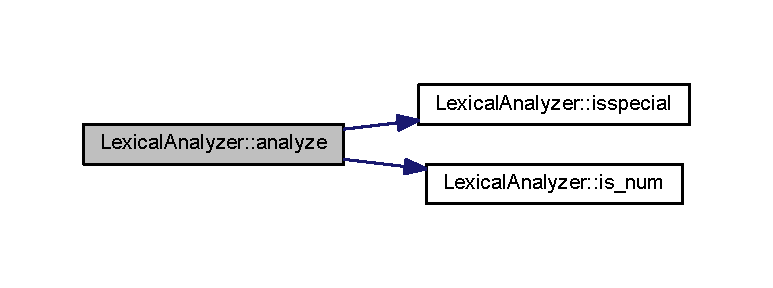
\includegraphics[width=350pt]{class_lexical_analyzer_afd35f07227fd40638e9d145ee6413640_cgraph}
\end{center}
\end{figure}




Граф вызова функции\+:
\nopagebreak
\begin{figure}[H]
\begin{center}
\leavevmode
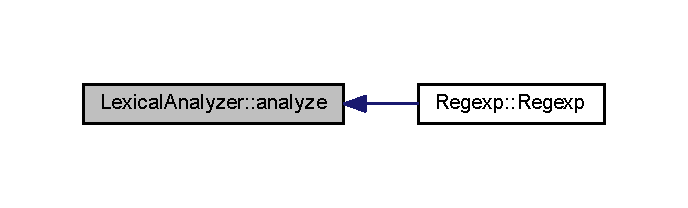
\includegraphics[width=330pt]{class_lexical_analyzer_afd35f07227fd40638e9d145ee6413640_icgraph}
\end{center}
\end{figure}


\index{Lexical\+Analyzer@{Lexical\+Analyzer}!is\+\_\+num@{is\+\_\+num}}
\index{is\+\_\+num@{is\+\_\+num}!Lexical\+Analyzer@{Lexical\+Analyzer}}
\subsubsection[{\texorpdfstring{is\+\_\+num(const string \&s)}{is_num(const string &s)}}]{\setlength{\rightskip}{0pt plus 5cm}string Lexical\+Analyzer\+::is\+\_\+num (
\begin{DoxyParamCaption}
\item[{const string \&}]{s}
\end{DoxyParamCaption}
)\hspace{0.3cm}{\ttfamily [static]}, {\ttfamily [private]}}\hypertarget{class_lexical_analyzer_a9e124ea0dcdfccc94f17ecc99aac6206}{}\label{class_lexical_analyzer_a9e124ea0dcdfccc94f17ecc99aac6206}
Проверяет, является ли строка числом 
\begin{DoxyParams}[1]{Аргументы}
\mbox{\tt in}  & {\em s} & Проверяемая строка\\
\hline
\end{DoxyParams}
\begin{DoxyReturn}{Возвращает}
Та же строка
\end{DoxyReturn}

\begin{DoxyExceptions}{Исключения}
{\em std\+::invalid\+\_\+argument} & В случае, если строка не является числом \\
\hline
{\em std\+::out\+\_\+of\+\_\+range} & В случае, если записанное в строке число не может поместиться в тип int \\
\hline
\end{DoxyExceptions}


Граф вызова функции\+:
\nopagebreak
\begin{figure}[H]
\begin{center}
\leavevmode
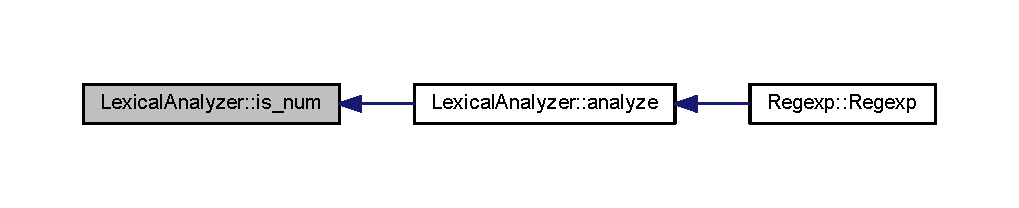
\includegraphics[width=350pt]{class_lexical_analyzer_a9e124ea0dcdfccc94f17ecc99aac6206_icgraph}
\end{center}
\end{figure}


\index{Lexical\+Analyzer@{Lexical\+Analyzer}!isspecial@{isspecial}}
\index{isspecial@{isspecial}!Lexical\+Analyzer@{Lexical\+Analyzer}}
\subsubsection[{\texorpdfstring{isspecial(char ch)}{isspecial(char ch)}}]{\setlength{\rightskip}{0pt plus 5cm}bool Lexical\+Analyzer\+::isspecial (
\begin{DoxyParamCaption}
\item[{char}]{ch}
\end{DoxyParamCaption}
)\hspace{0.3cm}{\ttfamily [static]}, {\ttfamily [private]}}\hypertarget{class_lexical_analyzer_a24d338442e8205f00690565bd2157ebc}{}\label{class_lexical_analyzer_a24d338442e8205f00690565bd2157ebc}
Проверяет, является ли символ специальным 
\begin{DoxyParams}[1]{Аргументы}
\mbox{\tt in}  & {\em ch} & Проверяемый символ\\
\hline
\end{DoxyParams}
\begin{DoxyReturn}{Возвращает}
Результат проверки 
\end{DoxyReturn}


Граф вызова функции\+:
\nopagebreak
\begin{figure}[H]
\begin{center}
\leavevmode
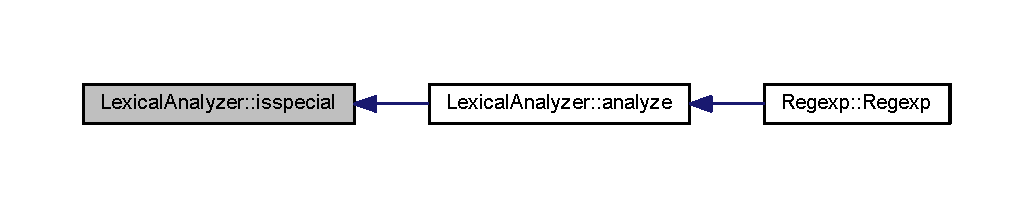
\includegraphics[width=350pt]{class_lexical_analyzer_a24d338442e8205f00690565bd2157ebc_icgraph}
\end{center}
\end{figure}




Объявления и описания членов классов находятся в файлах\+:\begin{DoxyCompactItemize}
\item 
\hyperlink{_lexical_analyzer_8h}{Lexical\+Analyzer.\+h}\item 
\hyperlink{_lexical_analyzer_8cpp}{Lexical\+Analyzer.\+cpp}\end{DoxyCompactItemize}

\hypertarget{structrc__result}{}\section{Структура rc\+\_\+result}
\label{structrc__result}\index{rc\+\_\+result@{rc\+\_\+result}}


Структура, описывающая формат результата  




{\ttfamily \#include $<$rc\+\_\+result.\+h$>$}

\subsection*{Открытые атрибуты}
\begin{DoxyCompactItemize}
\item 
bool \hyperlink{structrc__result_ab0d0340122026893c6b5fb577e71b015}{status}
\begin{DoxyCompactList}\small\item\em Результат проверки \end{DoxyCompactList}\item 
std\+::string \hyperlink{structrc__result_aa2797793b3623a02a09c29a60e9094ac}{result}
\begin{DoxyCompactList}\small\item\em Строка, используемая для хранения найденной подстроки \end{DoxyCompactList}\end{DoxyCompactItemize}


\subsection{Подробное описание}
Структура, описывающая формат результата 

\subsection{Данные класса}
\index{rc\+\_\+result@{rc\+\_\+result}!result@{result}}
\index{result@{result}!rc\+\_\+result@{rc\+\_\+result}}
\subsubsection[{\texorpdfstring{result}{result}}]{\setlength{\rightskip}{0pt plus 5cm}std\+::string rc\+\_\+result\+::result}\hypertarget{structrc__result_aa2797793b3623a02a09c29a60e9094ac}{}\label{structrc__result_aa2797793b3623a02a09c29a60e9094ac}


Строка, используемая для хранения найденной подстроки 

\index{rc\+\_\+result@{rc\+\_\+result}!status@{status}}
\index{status@{status}!rc\+\_\+result@{rc\+\_\+result}}
\subsubsection[{\texorpdfstring{status}{status}}]{\setlength{\rightskip}{0pt plus 5cm}bool rc\+\_\+result\+::status}\hypertarget{structrc__result_ab0d0340122026893c6b5fb577e71b015}{}\label{structrc__result_ab0d0340122026893c6b5fb577e71b015}


Результат проверки 



Объявления и описания членов структуры находятся в файле\+:\begin{DoxyCompactItemize}
\item 
\hyperlink{rc__result_8h}{rc\+\_\+result.\+h}\end{DoxyCompactItemize}

\hypertarget{class_regexp}{}\section{Класс Regexp}
\label{class_regexp}\index{Regexp@{Regexp}}


Класс регулярного выражения  




{\ttfamily \#include $<$Regexp.\+h$>$}

\subsection*{Открытые члены}
\begin{DoxyCompactItemize}
\item 
\hyperlink{class_regexp_abde3553b9033fd74f944dba8cdb6b9ea}{Regexp} (const string \&pattern)
\item 
\hyperlink{class_regexp_ada3dfc1370864a39089592fbe27ef19d}{$\sim$\+Regexp} ()
\item 
bool \hyperlink{class_regexp_a7869806d5707d47742db7ad5129b6585}{match} (const string \&target) const 
\item 
\hyperlink{structrc__result}{rc\+\_\+result} \hyperlink{class_regexp_af7c296f94f7577ce0fa662c78268659e}{search} (const string \&target) const 
\end{DoxyCompactItemize}
\subsection*{Закрытые данные}
\begin{DoxyCompactItemize}
\item 
vector$<$ \hyperlink{structtoken}{token} $>$ \hyperlink{class_regexp_a784da1e5f4f040a16734c9e3dee089a5}{sv}
\begin{DoxyCompactList}\small\item\em Вектор с преобразованными лексемами \end{DoxyCompactList}\end{DoxyCompactItemize}


\subsection{Подробное описание}
Класс регулярного выражения 

Класс регулярного выражения служит для проверки строк на соответствие регулярному выражению и поиска подстроки, соответствующей регулярному выржению, в заданной строке 

\subsection{Конструктор(ы)}
\index{Regexp@{Regexp}!Regexp@{Regexp}}
\index{Regexp@{Regexp}!Regexp@{Regexp}}
\subsubsection[{\texorpdfstring{Regexp(const string \&pattern)}{Regexp(const string &pattern)}}]{\setlength{\rightskip}{0pt plus 5cm}Regexp\+::\+Regexp (
\begin{DoxyParamCaption}
\item[{const string \&}]{pattern}
\end{DoxyParamCaption}
)}\hypertarget{class_regexp_abde3553b9033fd74f944dba8cdb6b9ea}{}\label{class_regexp_abde3553b9033fd74f944dba8cdb6b9ea}
Конструктор регулярного выражения 
\begin{DoxyParams}[1]{Аргументы}
\mbox{\tt in}  & {\em pattern} & Регулярное выражение в строковом виде \\
\hline
\end{DoxyParams}


Граф вызовов\+:
\nopagebreak
\begin{figure}[H]
\begin{center}
\leavevmode
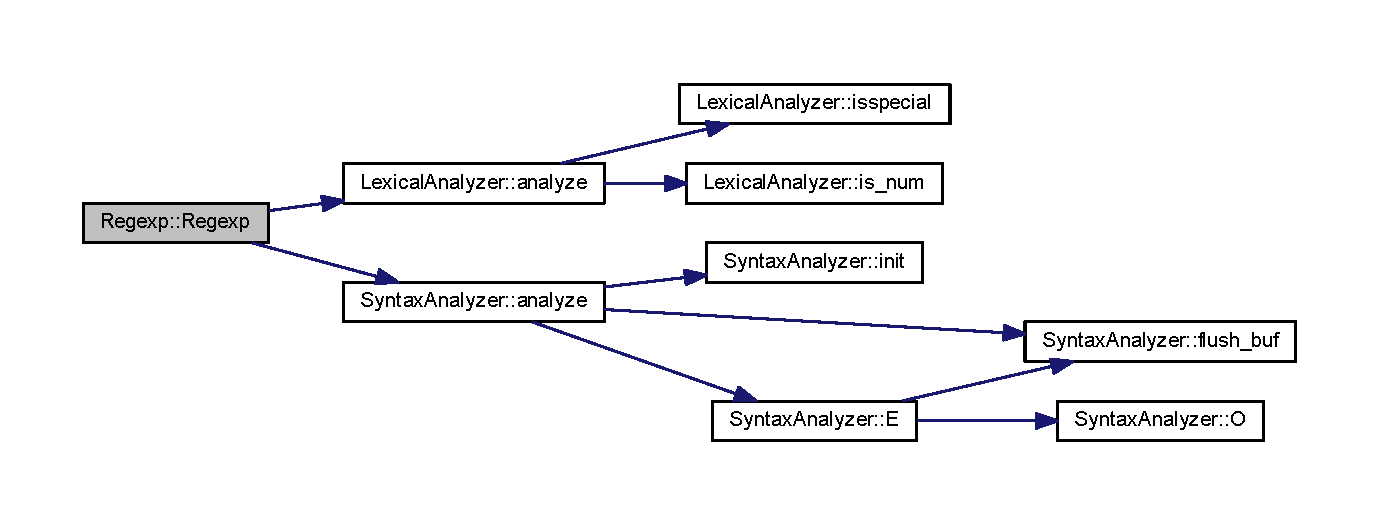
\includegraphics[width=350pt]{class_regexp_abde3553b9033fd74f944dba8cdb6b9ea_cgraph}
\end{center}
\end{figure}


\index{Regexp@{Regexp}!````~Regexp@{$\sim$\+Regexp}}
\index{````~Regexp@{$\sim$\+Regexp}!Regexp@{Regexp}}
\subsubsection[{\texorpdfstring{$\sim$\+Regexp()}{~Regexp()}}]{\setlength{\rightskip}{0pt plus 5cm}Regexp\+::$\sim$\+Regexp (
\begin{DoxyParamCaption}
{}
\end{DoxyParamCaption}
)\hspace{0.3cm}{\ttfamily [inline]}}\hypertarget{class_regexp_ada3dfc1370864a39089592fbe27ef19d}{}\label{class_regexp_ada3dfc1370864a39089592fbe27ef19d}


Граф вызовов\+:
\nopagebreak
\begin{figure}[H]
\begin{center}
\leavevmode
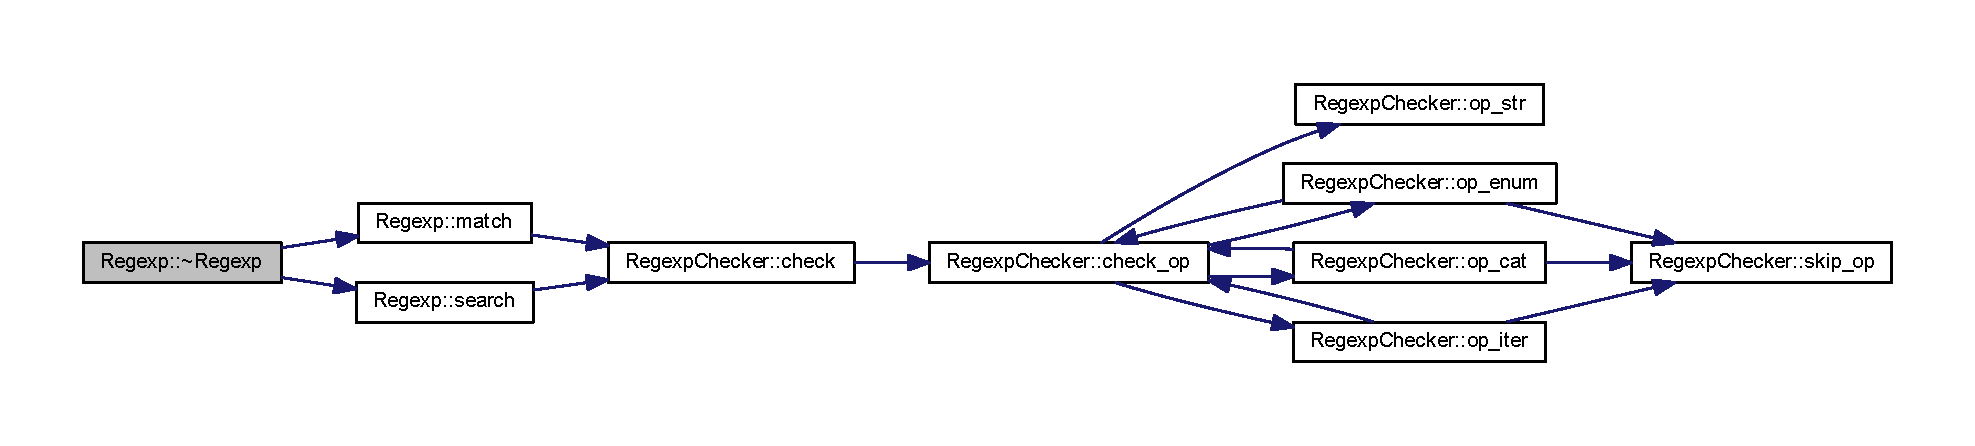
\includegraphics[width=350pt]{class_regexp_ada3dfc1370864a39089592fbe27ef19d_cgraph}
\end{center}
\end{figure}




\subsection{Методы}
\index{Regexp@{Regexp}!match@{match}}
\index{match@{match}!Regexp@{Regexp}}
\subsubsection[{\texorpdfstring{match(const string \&target) const }{match(const string &target) const }}]{\setlength{\rightskip}{0pt plus 5cm}bool Regexp\+::match (
\begin{DoxyParamCaption}
\item[{const string \&}]{target}
\end{DoxyParamCaption}
) const}\hypertarget{class_regexp_a7869806d5707d47742db7ad5129b6585}{}\label{class_regexp_a7869806d5707d47742db7ad5129b6585}
Проверяет строку на соответствие регулярному выражению 
\begin{DoxyParams}[1]{Аргументы}
\mbox{\tt in}  & {\em target} & Строка, которую необходимо проверить\\
\hline
\end{DoxyParams}
\begin{DoxyReturn}{Возвращает}
Результат проверки 
\end{DoxyReturn}


Граф вызовов\+:
\nopagebreak
\begin{figure}[H]
\begin{center}
\leavevmode
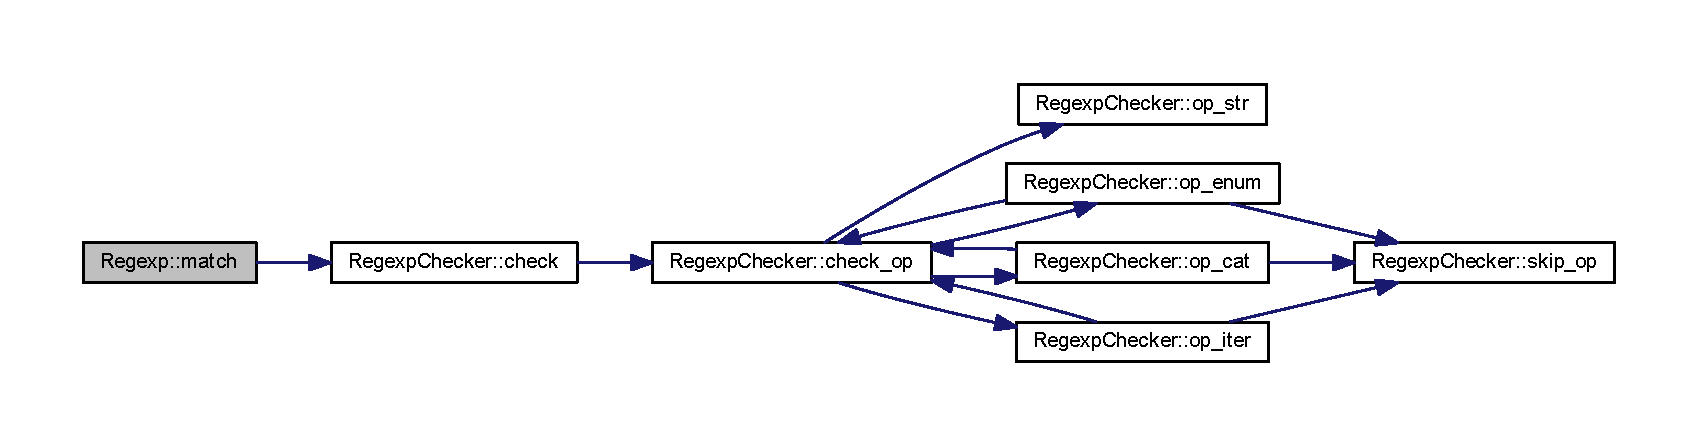
\includegraphics[width=350pt]{class_regexp_a7869806d5707d47742db7ad5129b6585_cgraph}
\end{center}
\end{figure}




Граф вызова функции\+:
\nopagebreak
\begin{figure}[H]
\begin{center}
\leavevmode
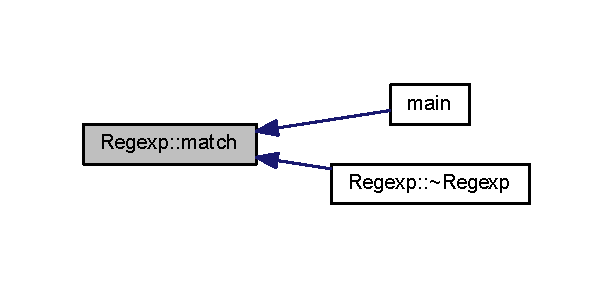
\includegraphics[width=294pt]{class_regexp_a7869806d5707d47742db7ad5129b6585_icgraph}
\end{center}
\end{figure}


\index{Regexp@{Regexp}!search@{search}}
\index{search@{search}!Regexp@{Regexp}}
\subsubsection[{\texorpdfstring{search(const string \&target) const }{search(const string &target) const }}]{\setlength{\rightskip}{0pt plus 5cm}{\bf rc\+\_\+result} Regexp\+::search (
\begin{DoxyParamCaption}
\item[{const string \&}]{target}
\end{DoxyParamCaption}
) const}\hypertarget{class_regexp_af7c296f94f7577ce0fa662c78268659e}{}\label{class_regexp_af7c296f94f7577ce0fa662c78268659e}
Ищет подстроку, соответствующую регулярному выражению, в строке 
\begin{DoxyParams}[1]{Аргументы}
\mbox{\tt in}  & {\em target} & Строка, в которой производится поиск\\
\hline
\end{DoxyParams}
\begin{DoxyReturn}{Возвращает}
Результат поиска 
\end{DoxyReturn}


Граф вызовов\+:
\nopagebreak
\begin{figure}[H]
\begin{center}
\leavevmode
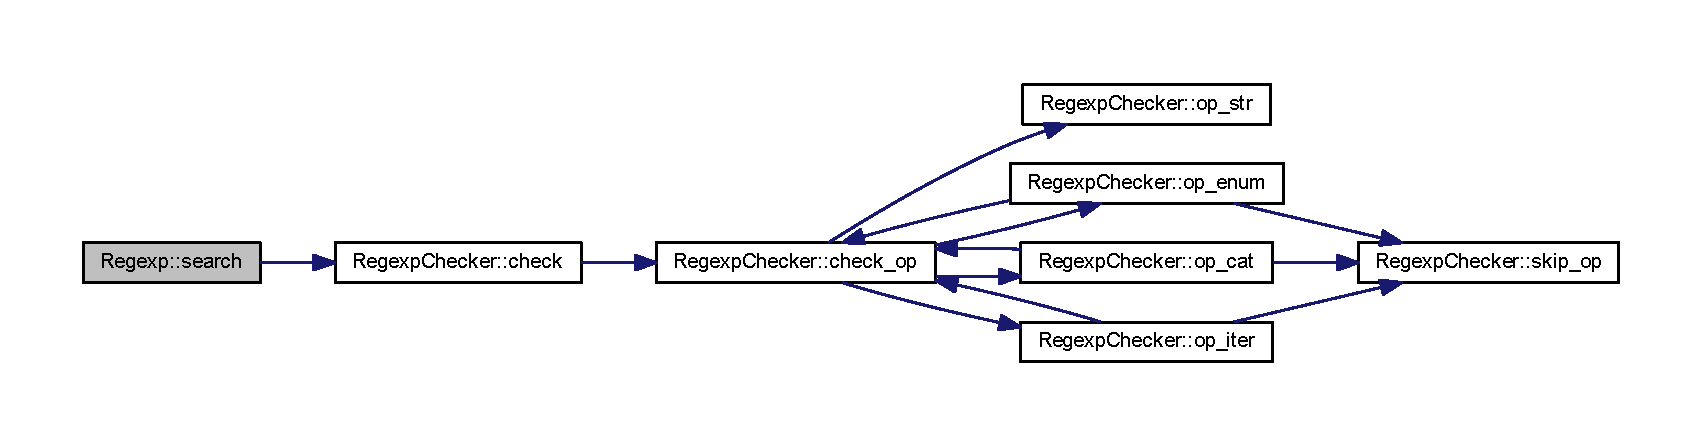
\includegraphics[width=350pt]{class_regexp_af7c296f94f7577ce0fa662c78268659e_cgraph}
\end{center}
\end{figure}




Граф вызова функции\+:
\nopagebreak
\begin{figure}[H]
\begin{center}
\leavevmode
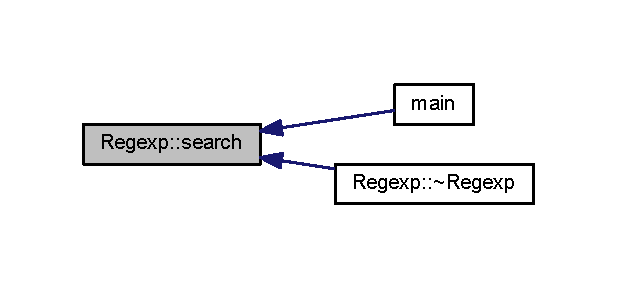
\includegraphics[width=296pt]{class_regexp_af7c296f94f7577ce0fa662c78268659e_icgraph}
\end{center}
\end{figure}




\subsection{Данные класса}
\index{Regexp@{Regexp}!sv@{sv}}
\index{sv@{sv}!Regexp@{Regexp}}
\subsubsection[{\texorpdfstring{sv}{sv}}]{\setlength{\rightskip}{0pt plus 5cm}vector$<${\bf token}$>$ Regexp\+::sv\hspace{0.3cm}{\ttfamily [private]}}\hypertarget{class_regexp_a784da1e5f4f040a16734c9e3dee089a5}{}\label{class_regexp_a784da1e5f4f040a16734c9e3dee089a5}


Вектор с преобразованными лексемами 



Объявления и описания членов классов находятся в файлах\+:\begin{DoxyCompactItemize}
\item 
\hyperlink{_regexp_8h}{Regexp.\+h}\item 
\hyperlink{_regexp_8cpp}{Regexp.\+cpp}\end{DoxyCompactItemize}

\hypertarget{class_regexp_checker}{}\section{Класс Regexp\+Checker}
\label{class_regexp_checker}\index{Regexp\+Checker@{Regexp\+Checker}}


Класс, проверяющий строку на соответствие регулярному выражению  




{\ttfamily \#include $<$Regexp\+Checker.\+h$>$}

\subsection*{Открытые члены}
\begin{DoxyCompactItemize}
\item 
\hyperlink{class_regexp_checker_a44a66429366e8d24ec92d07ea2f0e86f}{Regexp\+Checker} (const vector$<$ \hyperlink{structtoken}{token} $>$ $\ast$v, const string $\ast$s, string\+::const\+\_\+iterator sit, bool \hyperlink{class_regexp_checker_a76fa7992eddb6adcd63d9df0e5db1a92}{search}=false)
\item 
\hyperlink{class_regexp_checker_aa2e7c0de7bb85d60f905535f0d2a65e5}{$\sim$\+Regexp\+Checker} ()
\item 
\hyperlink{structrc__result}{rc\+\_\+result} \hyperlink{class_regexp_checker_a58d9c7c69c53ef18fa6ddb6a2c4bf24f}{check} ()
\end{DoxyCompactItemize}
\subsection*{Закрытые члены}
\begin{DoxyCompactItemize}
\item 
bool \hyperlink{class_regexp_checker_a12a12dfe322def2c802afd2ebea0b75f}{check\+\_\+op} ()
\item 
bool \hyperlink{class_regexp_checker_ad48539a0443212d78e32ff0a23918478}{op\+\_\+str} ()
\item 
bool \hyperlink{class_regexp_checker_aa775725022ae645c6d8f12633aa3a3d4}{op\+\_\+enum} ()
\item 
bool \hyperlink{class_regexp_checker_a3f379e2420eacf52f91afce6e0ade9e4}{op\+\_\+cat} ()
\item 
bool \hyperlink{class_regexp_checker_a5a34d99e02dba23757f33ce8107a961d}{op\+\_\+iter} (int min=0, int max=-\/1)
\item 
void \hyperlink{class_regexp_checker_adf00606a82e27c614122d001f21f9f96}{skip\+\_\+op} ()
\begin{DoxyCompactList}\small\item\em Пропускает текущую операцию \end{DoxyCompactList}\end{DoxyCompactItemize}
\subsection*{Закрытые данные}
\begin{DoxyCompactItemize}
\item 
bool \hyperlink{class_regexp_checker_a5003c015965ce4177450557c01543812}{child}
\begin{DoxyCompactList}\small\item\em Показывает, является ли даный процесс дочерним \end{DoxyCompactList}\item 
const vector$<$ \hyperlink{structtoken}{token} $>$ $\ast$ \hyperlink{class_regexp_checker_a4542347ee72d793d080b046be483d397}{sv}
\begin{DoxyCompactList}\small\item\em Указатель на вектор с преобразованными лексемами \end{DoxyCompactList}\item 
vector$<$ \hyperlink{structtoken}{token} $>$\+::const\+\_\+iterator \hyperlink{class_regexp_checker_a9823ceadabc26fe4c9042a86dddb4e34}{svit}
\begin{DoxyCompactList}\small\item\em Итератор, используемый для обхода вектора лексем \end{DoxyCompactList}\item 
const string $\ast$ \hyperlink{class_regexp_checker_a9a5672b777e0718a778e9061c3f579e6}{target}
\begin{DoxyCompactList}\small\item\em Указатель на строку, которую необходимо проверить \end{DoxyCompactList}\item 
const string\+::const\+\_\+iterator \hyperlink{class_regexp_checker_a54f557b93e0f498422185294726d129c}{btit}
\begin{DoxyCompactList}\small\item\em Итератор, указывающий на место в строке, с которого начинается проверка \end{DoxyCompactList}\item 
string\+::const\+\_\+iterator \hyperlink{class_regexp_checker_a782456d19baedddca76f23c3efd8cc53}{tit}
\begin{DoxyCompactList}\small\item\em Итератор, используемый для перемещения по строке \end{DoxyCompactList}\item 
bool \hyperlink{class_regexp_checker_a76fa7992eddb6adcd63d9df0e5db1a92}{search}
\begin{DoxyCompactList}\small\item\em Показывает, находится ли класс в режиме поиска подстроки \end{DoxyCompactList}\end{DoxyCompactItemize}


\subsection{Подробное описание}
Класс, проверяющий строку на соответствие регулярному выражению 

Класс последовательно выполняет операции регулярного выражения, с учётом их приоритетов, проверяя таким образом строку на соответствие 

\subsection{Конструктор(ы)}
\index{Regexp\+Checker@{Regexp\+Checker}!Regexp\+Checker@{Regexp\+Checker}}
\index{Regexp\+Checker@{Regexp\+Checker}!Regexp\+Checker@{Regexp\+Checker}}
\subsubsection[{\texorpdfstring{Regexp\+Checker(const vector$<$ token $>$ $\ast$v, const string $\ast$s, string\+::const\+\_\+iterator sit, bool search=false)}{RegexpChecker(const vector< token > *v, const string *s, string::const_iterator sit, bool search=false)}}]{\setlength{\rightskip}{0pt plus 5cm}Regexp\+Checker\+::\+Regexp\+Checker (
\begin{DoxyParamCaption}
\item[{const vector$<$ {\bf token} $>$ $\ast$}]{v, }
\item[{const string $\ast$}]{s, }
\item[{string\+::const\+\_\+iterator}]{sit, }
\item[{bool}]{search = {\ttfamily false}}
\end{DoxyParamCaption}
)}\hypertarget{class_regexp_checker_a44a66429366e8d24ec92d07ea2f0e86f}{}\label{class_regexp_checker_a44a66429366e8d24ec92d07ea2f0e86f}
Конструктор класса 
\begin{DoxyParams}[1]{Аргументы}
\mbox{\tt in}  & {\em v} & Указатель на вектор лексем регулярного выражения в префиксной форме \\
\hline
\mbox{\tt in}  & {\em s} & Указатель на строку, которую необходимо проверить \\
\hline
\mbox{\tt in}  & {\em sit} & Итератор, который используется для задания начальной позиции для обработки строки \\
\hline
\mbox{\tt in}  & {\em search} & Определяет режим проверки\+: сопоставление или поиск \\
\hline
\end{DoxyParams}
\index{Regexp\+Checker@{Regexp\+Checker}!````~Regexp\+Checker@{$\sim$\+Regexp\+Checker}}
\index{````~Regexp\+Checker@{$\sim$\+Regexp\+Checker}!Regexp\+Checker@{Regexp\+Checker}}
\subsubsection[{\texorpdfstring{$\sim$\+Regexp\+Checker()}{~RegexpChecker()}}]{\setlength{\rightskip}{0pt plus 5cm}Regexp\+Checker\+::$\sim$\+Regexp\+Checker (
\begin{DoxyParamCaption}
{}
\end{DoxyParamCaption}
)\hspace{0.3cm}{\ttfamily [inline]}}\hypertarget{class_regexp_checker_aa2e7c0de7bb85d60f905535f0d2a65e5}{}\label{class_regexp_checker_aa2e7c0de7bb85d60f905535f0d2a65e5}


\subsection{Методы}
\index{Regexp\+Checker@{Regexp\+Checker}!check@{check}}
\index{check@{check}!Regexp\+Checker@{Regexp\+Checker}}
\subsubsection[{\texorpdfstring{check()}{check()}}]{\setlength{\rightskip}{0pt plus 5cm}{\bf rc\+\_\+result} Regexp\+Checker\+::check (
\begin{DoxyParamCaption}
{}
\end{DoxyParamCaption}
)}\hypertarget{class_regexp_checker_a58d9c7c69c53ef18fa6ddb6a2c4bf24f}{}\label{class_regexp_checker_a58d9c7c69c53ef18fa6ddb6a2c4bf24f}
Запускает проверку

\begin{DoxyReturn}{Возвращает}
Результат проверки 
\end{DoxyReturn}


Граф вызовов\+:
\nopagebreak
\begin{figure}[H]
\begin{center}
\leavevmode
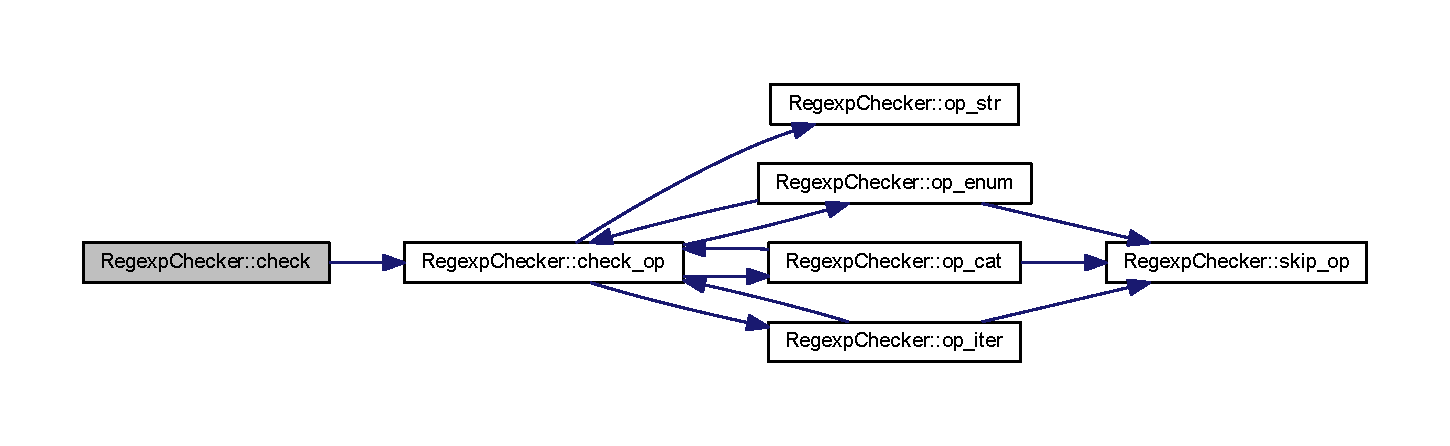
\includegraphics[width=350pt]{class_regexp_checker_a58d9c7c69c53ef18fa6ddb6a2c4bf24f_cgraph}
\end{center}
\end{figure}




Граф вызова функции\+:
\nopagebreak
\begin{figure}[H]
\begin{center}
\leavevmode
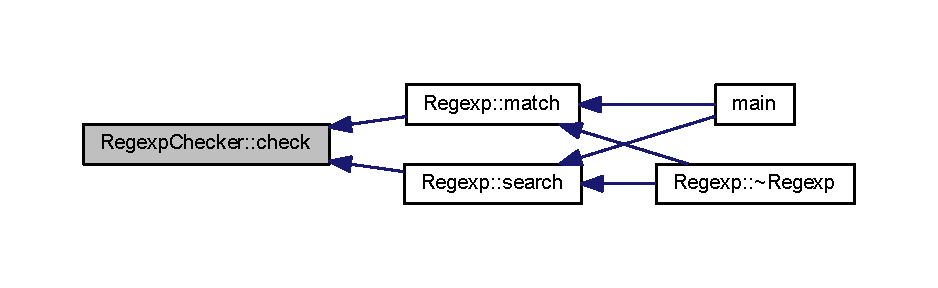
\includegraphics[width=350pt]{class_regexp_checker_a58d9c7c69c53ef18fa6ddb6a2c4bf24f_icgraph}
\end{center}
\end{figure}


\index{Regexp\+Checker@{Regexp\+Checker}!check\+\_\+op@{check\+\_\+op}}
\index{check\+\_\+op@{check\+\_\+op}!Regexp\+Checker@{Regexp\+Checker}}
\subsubsection[{\texorpdfstring{check\+\_\+op()}{check_op()}}]{\setlength{\rightskip}{0pt plus 5cm}bool Regexp\+Checker\+::check\+\_\+op (
\begin{DoxyParamCaption}
{}
\end{DoxyParamCaption}
)\hspace{0.3cm}{\ttfamily [private]}}\hypertarget{class_regexp_checker_a12a12dfe322def2c802afd2ebea0b75f}{}\label{class_regexp_checker_a12a12dfe322def2c802afd2ebea0b75f}
Выполняет текующую операцию

\begin{DoxyReturn}{Возвращает}
Результат операции 
\end{DoxyReturn}


Граф вызовов\+:
\nopagebreak
\begin{figure}[H]
\begin{center}
\leavevmode
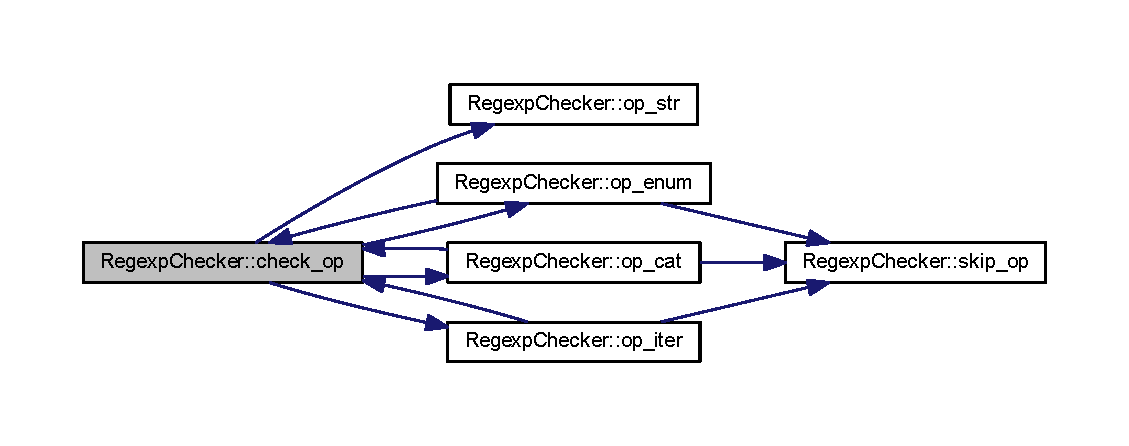
\includegraphics[width=350pt]{class_regexp_checker_a12a12dfe322def2c802afd2ebea0b75f_cgraph}
\end{center}
\end{figure}




Граф вызова функции\+:
\nopagebreak
\begin{figure}[H]
\begin{center}
\leavevmode
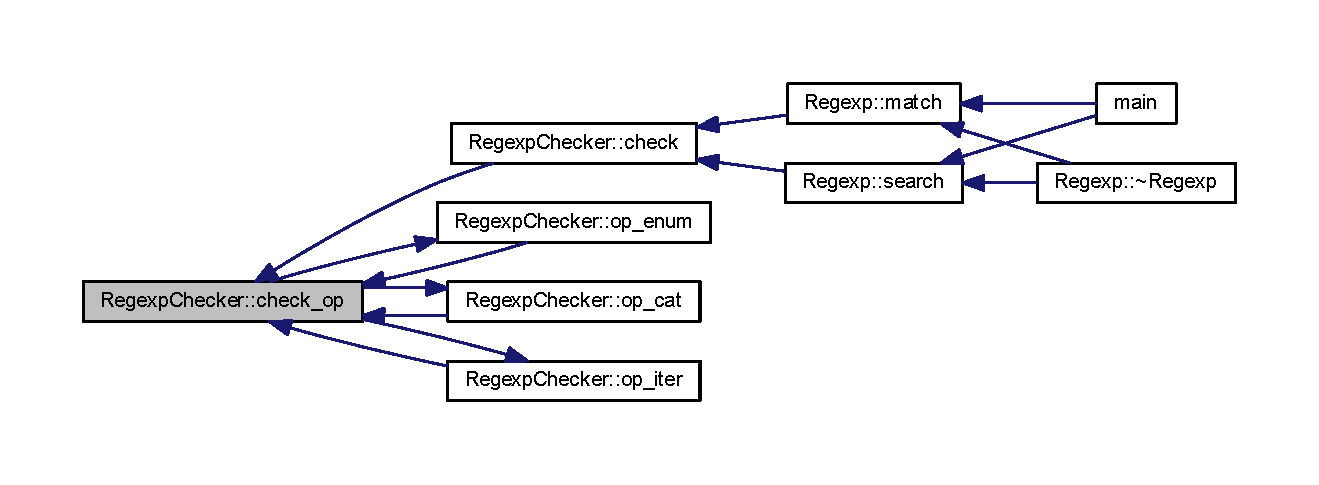
\includegraphics[width=350pt]{class_regexp_checker_a12a12dfe322def2c802afd2ebea0b75f_icgraph}
\end{center}
\end{figure}


\index{Regexp\+Checker@{Regexp\+Checker}!op\+\_\+cat@{op\+\_\+cat}}
\index{op\+\_\+cat@{op\+\_\+cat}!Regexp\+Checker@{Regexp\+Checker}}
\subsubsection[{\texorpdfstring{op\+\_\+cat()}{op_cat()}}]{\setlength{\rightskip}{0pt plus 5cm}bool Regexp\+Checker\+::op\+\_\+cat (
\begin{DoxyParamCaption}
{}
\end{DoxyParamCaption}
)\hspace{0.3cm}{\ttfamily [private]}}\hypertarget{class_regexp_checker_a3f379e2420eacf52f91afce6e0ade9e4}{}\label{class_regexp_checker_a3f379e2420eacf52f91afce6e0ade9e4}
Выполняет операцию конкатенации

\begin{DoxyReturn}{Возвращает}
Результат операции 
\end{DoxyReturn}


Граф вызовов\+:
\nopagebreak
\begin{figure}[H]
\begin{center}
\leavevmode
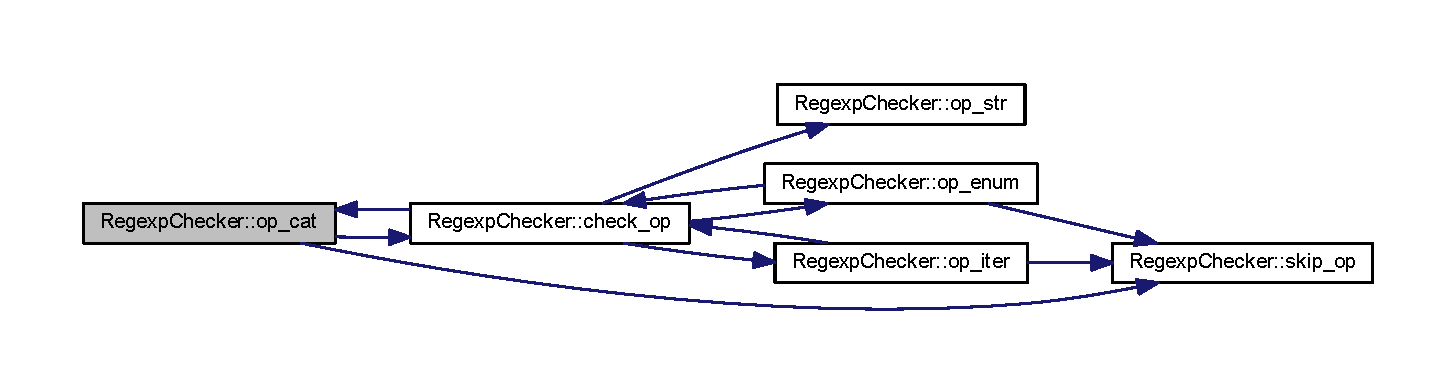
\includegraphics[width=350pt]{class_regexp_checker_a3f379e2420eacf52f91afce6e0ade9e4_cgraph}
\end{center}
\end{figure}




Граф вызова функции\+:
\nopagebreak
\begin{figure}[H]
\begin{center}
\leavevmode
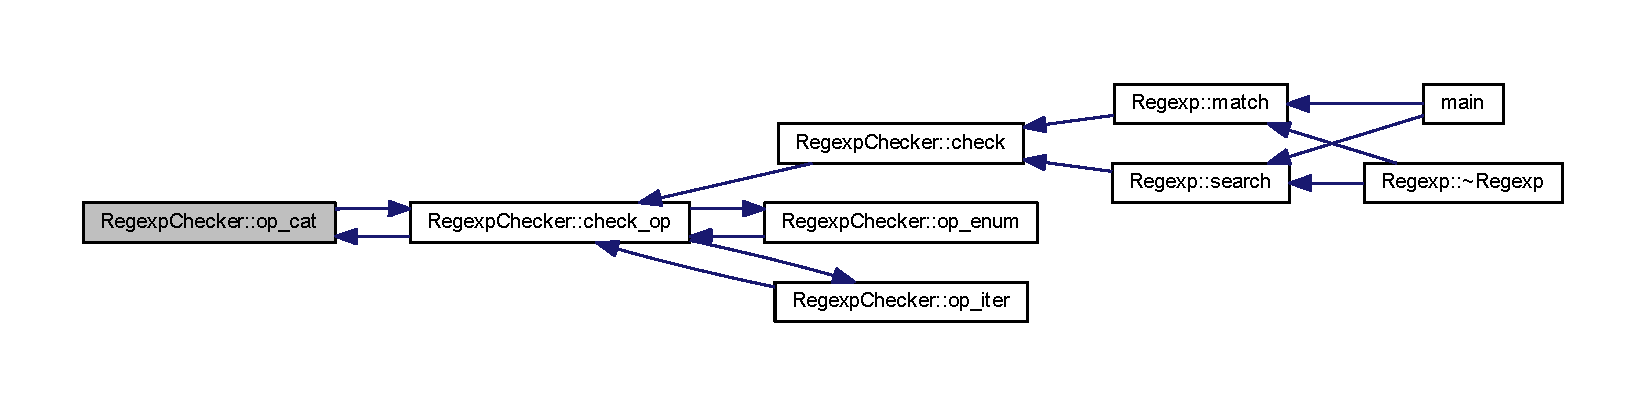
\includegraphics[width=350pt]{class_regexp_checker_a3f379e2420eacf52f91afce6e0ade9e4_icgraph}
\end{center}
\end{figure}


\index{Regexp\+Checker@{Regexp\+Checker}!op\+\_\+enum@{op\+\_\+enum}}
\index{op\+\_\+enum@{op\+\_\+enum}!Regexp\+Checker@{Regexp\+Checker}}
\subsubsection[{\texorpdfstring{op\+\_\+enum()}{op_enum()}}]{\setlength{\rightskip}{0pt plus 5cm}bool Regexp\+Checker\+::op\+\_\+enum (
\begin{DoxyParamCaption}
{}
\end{DoxyParamCaption}
)\hspace{0.3cm}{\ttfamily [private]}}\hypertarget{class_regexp_checker_aa775725022ae645c6d8f12633aa3a3d4}{}\label{class_regexp_checker_aa775725022ae645c6d8f12633aa3a3d4}
Выполняет операцию перечисления

\begin{DoxyReturn}{Возвращает}
Результат операции 
\end{DoxyReturn}


Граф вызовов\+:
\nopagebreak
\begin{figure}[H]
\begin{center}
\leavevmode
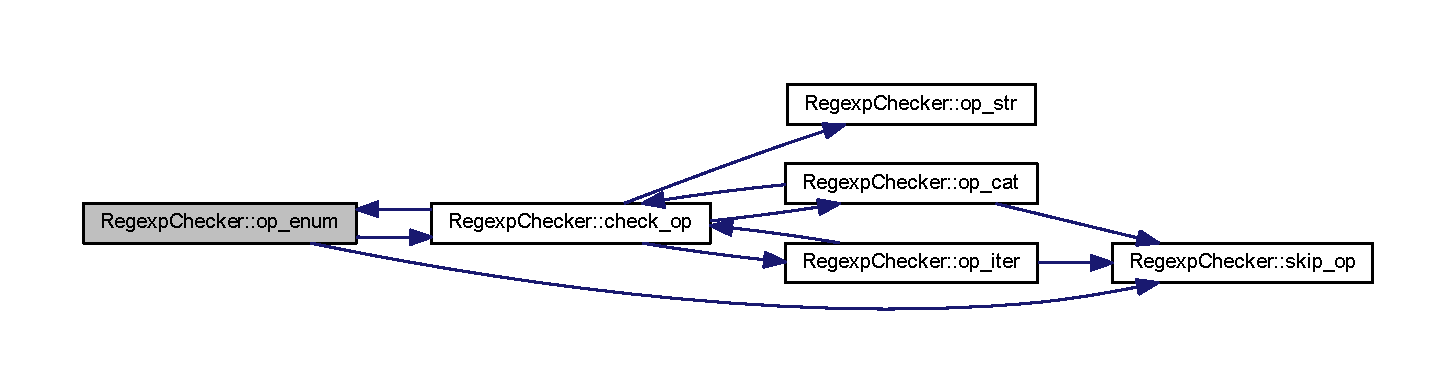
\includegraphics[width=350pt]{class_regexp_checker_aa775725022ae645c6d8f12633aa3a3d4_cgraph}
\end{center}
\end{figure}




Граф вызова функции\+:
\nopagebreak
\begin{figure}[H]
\begin{center}
\leavevmode
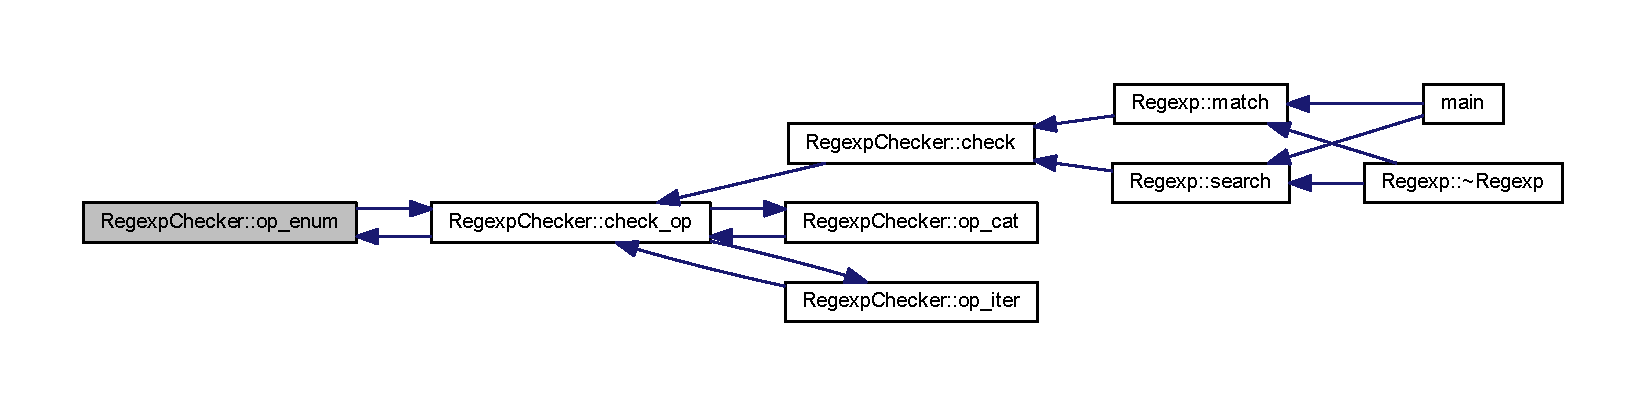
\includegraphics[width=350pt]{class_regexp_checker_aa775725022ae645c6d8f12633aa3a3d4_icgraph}
\end{center}
\end{figure}


\index{Regexp\+Checker@{Regexp\+Checker}!op\+\_\+iter@{op\+\_\+iter}}
\index{op\+\_\+iter@{op\+\_\+iter}!Regexp\+Checker@{Regexp\+Checker}}
\subsubsection[{\texorpdfstring{op\+\_\+iter(int min=0, int max=-\/1)}{op_iter(int min=0, int max=-1)}}]{\setlength{\rightskip}{0pt plus 5cm}bool Regexp\+Checker\+::op\+\_\+iter (
\begin{DoxyParamCaption}
\item[{int}]{min = {\ttfamily 0}, }
\item[{int}]{max = {\ttfamily -\/1}}
\end{DoxyParamCaption}
)\hspace{0.3cm}{\ttfamily [private]}}\hypertarget{class_regexp_checker_a5a34d99e02dba23757f33ce8107a961d}{}\label{class_regexp_checker_a5a34d99e02dba23757f33ce8107a961d}
Выполняет операцию итерирования 
\begin{DoxyParams}[1]{Аргументы}
\mbox{\tt in}  & {\em min} & Минимально необходимое количество итераций \\
\hline
\mbox{\tt in}  & {\em max} & Максимальное количество итераций\\
\hline
\end{DoxyParams}
\begin{DoxyReturn}{Возвращает}
Результат операции 
\end{DoxyReturn}


Граф вызовов\+:
\nopagebreak
\begin{figure}[H]
\begin{center}
\leavevmode
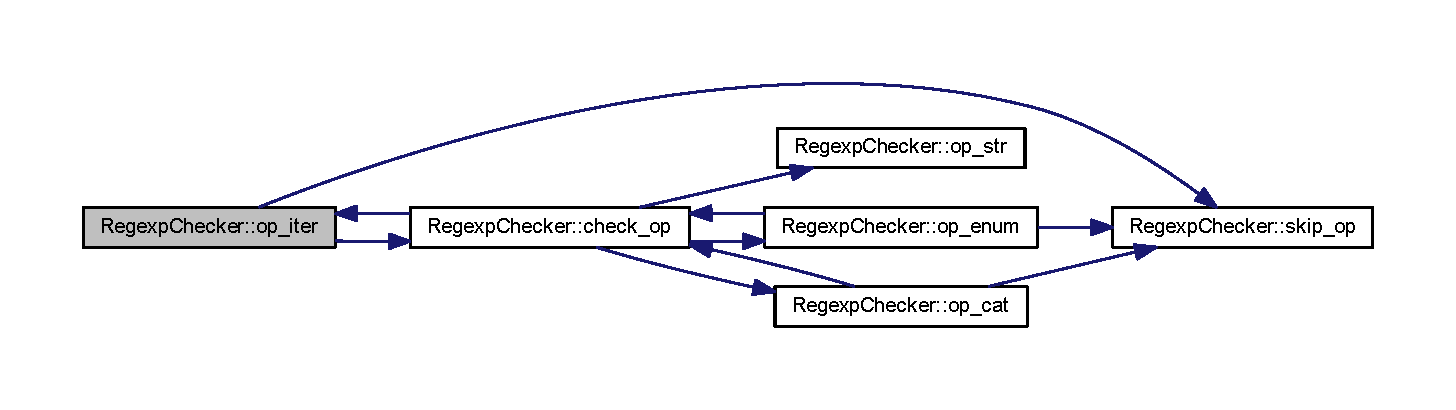
\includegraphics[width=350pt]{class_regexp_checker_a5a34d99e02dba23757f33ce8107a961d_cgraph}
\end{center}
\end{figure}




Граф вызова функции\+:
\nopagebreak
\begin{figure}[H]
\begin{center}
\leavevmode
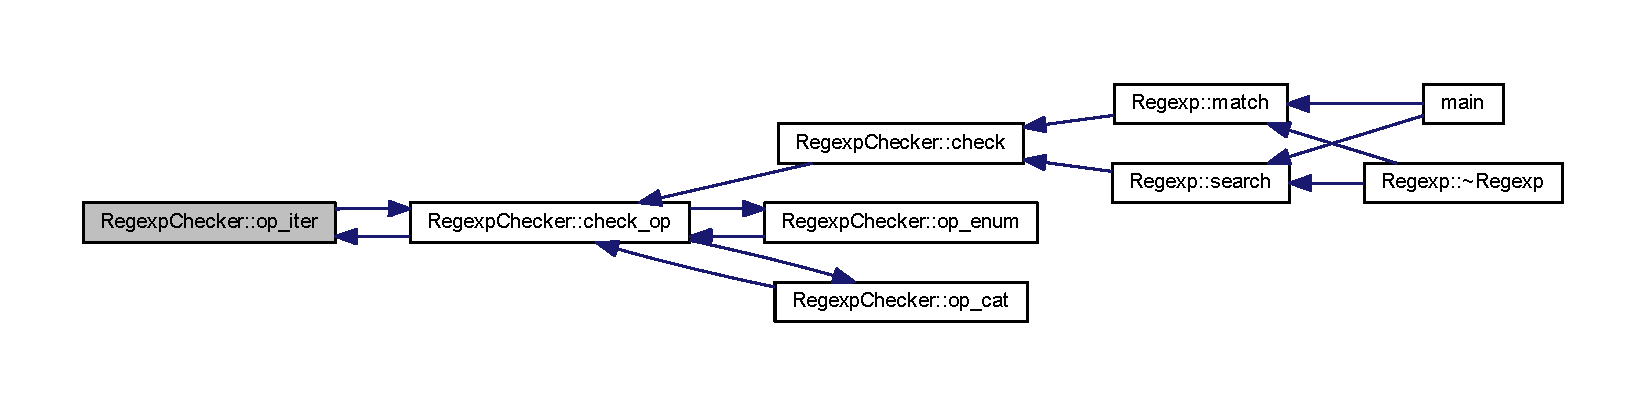
\includegraphics[width=350pt]{class_regexp_checker_a5a34d99e02dba23757f33ce8107a961d_icgraph}
\end{center}
\end{figure}


\index{Regexp\+Checker@{Regexp\+Checker}!op\+\_\+str@{op\+\_\+str}}
\index{op\+\_\+str@{op\+\_\+str}!Regexp\+Checker@{Regexp\+Checker}}
\subsubsection[{\texorpdfstring{op\+\_\+str()}{op_str()}}]{\setlength{\rightskip}{0pt plus 5cm}bool Regexp\+Checker\+::op\+\_\+str (
\begin{DoxyParamCaption}
{}
\end{DoxyParamCaption}
)\hspace{0.3cm}{\ttfamily [private]}}\hypertarget{class_regexp_checker_ad48539a0443212d78e32ff0a23918478}{}\label{class_regexp_checker_ad48539a0443212d78e32ff0a23918478}
Проверяет на соответствие последовательность литералов

\begin{DoxyReturn}{Возвращает}
Результат операции 
\end{DoxyReturn}


Граф вызова функции\+:
\nopagebreak
\begin{figure}[H]
\begin{center}
\leavevmode
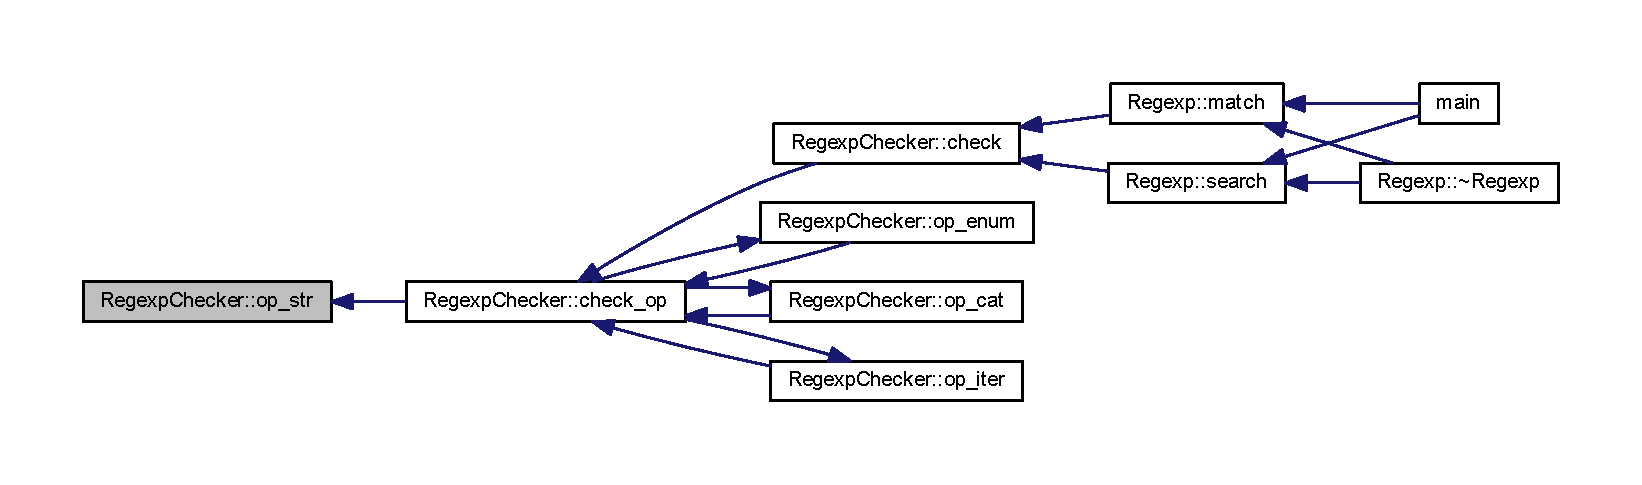
\includegraphics[width=350pt]{class_regexp_checker_ad48539a0443212d78e32ff0a23918478_icgraph}
\end{center}
\end{figure}


\index{Regexp\+Checker@{Regexp\+Checker}!skip\+\_\+op@{skip\+\_\+op}}
\index{skip\+\_\+op@{skip\+\_\+op}!Regexp\+Checker@{Regexp\+Checker}}
\subsubsection[{\texorpdfstring{skip\+\_\+op()}{skip_op()}}]{\setlength{\rightskip}{0pt plus 5cm}void Regexp\+Checker\+::skip\+\_\+op (
\begin{DoxyParamCaption}
{}
\end{DoxyParamCaption}
)\hspace{0.3cm}{\ttfamily [private]}}\hypertarget{class_regexp_checker_adf00606a82e27c614122d001f21f9f96}{}\label{class_regexp_checker_adf00606a82e27c614122d001f21f9f96}


Пропускает текущую операцию 



Граф вызова функции\+:
\nopagebreak
\begin{figure}[H]
\begin{center}
\leavevmode
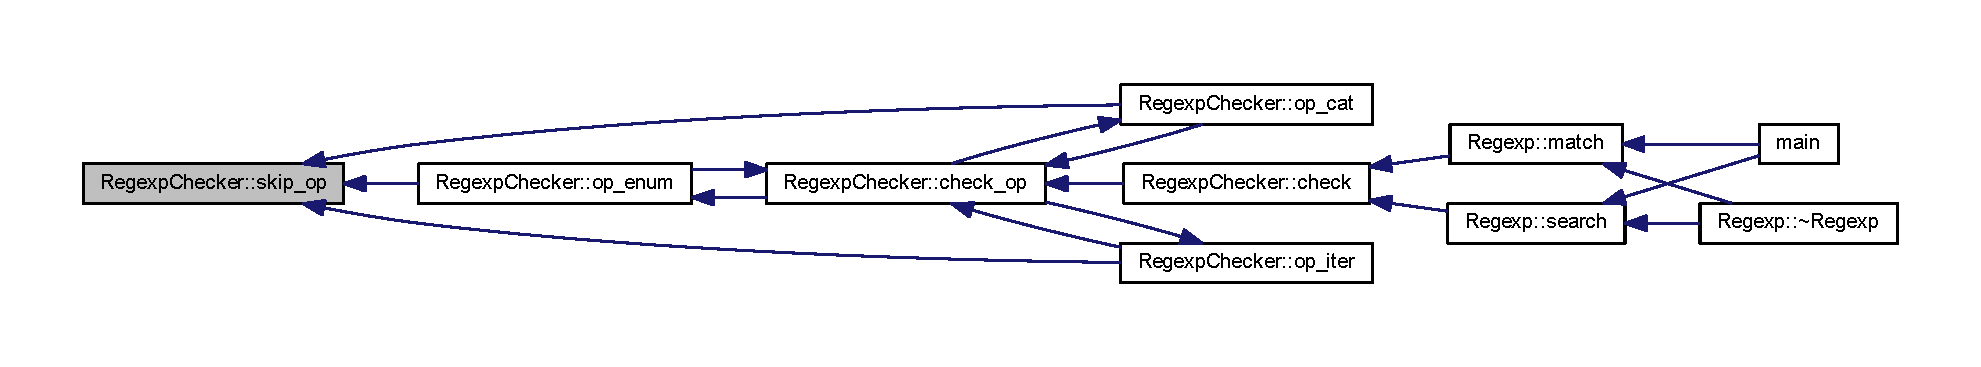
\includegraphics[width=350pt]{class_regexp_checker_adf00606a82e27c614122d001f21f9f96_icgraph}
\end{center}
\end{figure}




\subsection{Данные класса}
\index{Regexp\+Checker@{Regexp\+Checker}!btit@{btit}}
\index{btit@{btit}!Regexp\+Checker@{Regexp\+Checker}}
\subsubsection[{\texorpdfstring{btit}{btit}}]{\setlength{\rightskip}{0pt plus 5cm}const string\+::const\+\_\+iterator Regexp\+Checker\+::btit\hspace{0.3cm}{\ttfamily [private]}}\hypertarget{class_regexp_checker_a54f557b93e0f498422185294726d129c}{}\label{class_regexp_checker_a54f557b93e0f498422185294726d129c}


Итератор, указывающий на место в строке, с которого начинается проверка 

\index{Regexp\+Checker@{Regexp\+Checker}!child@{child}}
\index{child@{child}!Regexp\+Checker@{Regexp\+Checker}}
\subsubsection[{\texorpdfstring{child}{child}}]{\setlength{\rightskip}{0pt plus 5cm}bool Regexp\+Checker\+::child\hspace{0.3cm}{\ttfamily [private]}}\hypertarget{class_regexp_checker_a5003c015965ce4177450557c01543812}{}\label{class_regexp_checker_a5003c015965ce4177450557c01543812}


Показывает, является ли даный процесс дочерним 

\index{Regexp\+Checker@{Regexp\+Checker}!search@{search}}
\index{search@{search}!Regexp\+Checker@{Regexp\+Checker}}
\subsubsection[{\texorpdfstring{search}{search}}]{\setlength{\rightskip}{0pt plus 5cm}bool Regexp\+Checker\+::search\hspace{0.3cm}{\ttfamily [private]}}\hypertarget{class_regexp_checker_a76fa7992eddb6adcd63d9df0e5db1a92}{}\label{class_regexp_checker_a76fa7992eddb6adcd63d9df0e5db1a92}


Показывает, находится ли класс в режиме поиска подстроки 

\index{Regexp\+Checker@{Regexp\+Checker}!sv@{sv}}
\index{sv@{sv}!Regexp\+Checker@{Regexp\+Checker}}
\subsubsection[{\texorpdfstring{sv}{sv}}]{\setlength{\rightskip}{0pt plus 5cm}const vector$<${\bf token}$>$$\ast$ Regexp\+Checker\+::sv\hspace{0.3cm}{\ttfamily [private]}}\hypertarget{class_regexp_checker_a4542347ee72d793d080b046be483d397}{}\label{class_regexp_checker_a4542347ee72d793d080b046be483d397}


Указатель на вектор с преобразованными лексемами 

\index{Regexp\+Checker@{Regexp\+Checker}!svit@{svit}}
\index{svit@{svit}!Regexp\+Checker@{Regexp\+Checker}}
\subsubsection[{\texorpdfstring{svit}{svit}}]{\setlength{\rightskip}{0pt plus 5cm}vector$<${\bf token}$>$\+::const\+\_\+iterator Regexp\+Checker\+::svit\hspace{0.3cm}{\ttfamily [private]}}\hypertarget{class_regexp_checker_a9823ceadabc26fe4c9042a86dddb4e34}{}\label{class_regexp_checker_a9823ceadabc26fe4c9042a86dddb4e34}


Итератор, используемый для обхода вектора лексем 

\index{Regexp\+Checker@{Regexp\+Checker}!target@{target}}
\index{target@{target}!Regexp\+Checker@{Regexp\+Checker}}
\subsubsection[{\texorpdfstring{target}{target}}]{\setlength{\rightskip}{0pt plus 5cm}const string$\ast$ Regexp\+Checker\+::target\hspace{0.3cm}{\ttfamily [private]}}\hypertarget{class_regexp_checker_a9a5672b777e0718a778e9061c3f579e6}{}\label{class_regexp_checker_a9a5672b777e0718a778e9061c3f579e6}


Указатель на строку, которую необходимо проверить 

\index{Regexp\+Checker@{Regexp\+Checker}!tit@{tit}}
\index{tit@{tit}!Regexp\+Checker@{Regexp\+Checker}}
\subsubsection[{\texorpdfstring{tit}{tit}}]{\setlength{\rightskip}{0pt plus 5cm}string\+::const\+\_\+iterator Regexp\+Checker\+::tit\hspace{0.3cm}{\ttfamily [private]}}\hypertarget{class_regexp_checker_a782456d19baedddca76f23c3efd8cc53}{}\label{class_regexp_checker_a782456d19baedddca76f23c3efd8cc53}


Итератор, используемый для перемещения по строке 



Объявления и описания членов классов находятся в файлах\+:\begin{DoxyCompactItemize}
\item 
\hyperlink{_regexp_checker_8h}{Regexp\+Checker.\+h}\item 
\hyperlink{_regexp_checker_8cpp}{Regexp\+Checker.\+cpp}\end{DoxyCompactItemize}

\hypertarget{class_syntax_analyzer}{}\section{Класс Syntax\+Analyzer}
\label{class_syntax_analyzer}\index{Syntax\+Analyzer@{Syntax\+Analyzer}}


Синтаксический анализатор  




{\ttfamily \#include $<$Syntax\+Analyzer.\+h$>$}

\subsection*{Открытые члены}
\begin{DoxyCompactItemize}
\item 
\hyperlink{class_syntax_analyzer_af4bb6b4b5a638914d5851082dd7a1669}{Syntax\+Analyzer} (const vector$<$ \hyperlink{structtoken}{token} $>$ \&tokens)
\item 
\hyperlink{class_syntax_analyzer_a29b52995ad07154244f129673dae5a01}{$\sim$\+Syntax\+Analyzer} ()
\item 
vector$<$ \hyperlink{structtoken}{token} $>$ \hyperlink{class_syntax_analyzer_a04fbf355b2afe30ef814048ecb029cf2}{analyze} ()
\end{DoxyCompactItemize}
\subsection*{Закрытые члены}
\begin{DoxyCompactItemize}
\item 
void \hyperlink{class_syntax_analyzer_a76c8c49d5154b9b48b11d241577420e4}{init} ()
\begin{DoxyCompactList}\small\item\em Инициализирует анализатор \end{DoxyCompactList}\item 
void \hyperlink{class_syntax_analyzer_a1b42fab3f30284bf29a7eff2f3e8382f}{E} (bool last=false)
\item 
bool \hyperlink{class_syntax_analyzer_a7a94734bb42224681a23045c45cd9ca3}{O} (int pos=-\/1)
\item 
bool \hyperlink{class_syntax_analyzer_aea363db29fd359d98711018d377f3301}{flush\+\_\+buf} (int pos=-\/1)
\end{DoxyCompactItemize}
\subsection*{Закрытые данные}
\begin{DoxyCompactItemize}
\item 
vector$<$ \hyperlink{structtoken}{token} $>$ \hyperlink{class_syntax_analyzer_aea5a27bee70623ed8bf91972938d39af}{raw\+\_\+tokens}
\begin{DoxyCompactList}\small\item\em Вектор исходных лексем \end{DoxyCompactList}\item 
vector$<$ \hyperlink{structtoken}{token} $>$ \hyperlink{class_syntax_analyzer_aadc7ff59a663670756f4ab5e81f7d99a}{pf\+\_\+tokens}
\begin{DoxyCompactList}\small\item\em Вектор с преобразованными лексемами \end{DoxyCompactList}\item 
vector$<$ \hyperlink{structtoken}{token} $>$\+::iterator \hyperlink{class_syntax_analyzer_a38e0d3b67ddaa431c1b200f2ad383e61}{it}
\begin{DoxyCompactList}\small\item\em Итератор, используемый для обхода вектора исходных лексем \end{DoxyCompactList}\item 
int \hyperlink{class_syntax_analyzer_a9ad8571c7819ba91db174772d3fbfbd9}{brackets\+\_\+count}
\begin{DoxyCompactList}\small\item\em Количество незакрытых скобок \end{DoxyCompactList}\item 
string \hyperlink{class_syntax_analyzer_a5b6fe22c4940c5560de49bebe38768e8}{buf}
\begin{DoxyCompactList}\small\item\em Буфер, используемый для объединения подряд идущих последовательностей литералов \end{DoxyCompactList}\end{DoxyCompactItemize}


\subsection{Подробное описание}
Синтаксический анализатор 

Синтаксический анализатор преобразует последовательность лексем, полученную от лексического анализатора, в префиксную форму, проверяя синтаксис регулярного выражения 

\subsection{Конструктор(ы)}
\index{Syntax\+Analyzer@{Syntax\+Analyzer}!Syntax\+Analyzer@{Syntax\+Analyzer}}
\index{Syntax\+Analyzer@{Syntax\+Analyzer}!Syntax\+Analyzer@{Syntax\+Analyzer}}
\subsubsection[{\texorpdfstring{Syntax\+Analyzer(const vector$<$ token $>$ \&tokens)}{SyntaxAnalyzer(const vector< token > &tokens)}}]{\setlength{\rightskip}{0pt plus 5cm}Syntax\+Analyzer\+::\+Syntax\+Analyzer (
\begin{DoxyParamCaption}
\item[{const vector$<$ {\bf token} $>$ \&}]{tokens}
\end{DoxyParamCaption}
)}\hypertarget{class_syntax_analyzer_af4bb6b4b5a638914d5851082dd7a1669}{}\label{class_syntax_analyzer_af4bb6b4b5a638914d5851082dd7a1669}
Конструктор синтаксического анализатора 
\begin{DoxyParams}[1]{Аргументы}
\mbox{\tt in}  & {\em tokens} & Вектор лексем, подлежащий обработке \\
\hline
\end{DoxyParams}


Граф вызовов\+:
\nopagebreak
\begin{figure}[H]
\begin{center}
\leavevmode
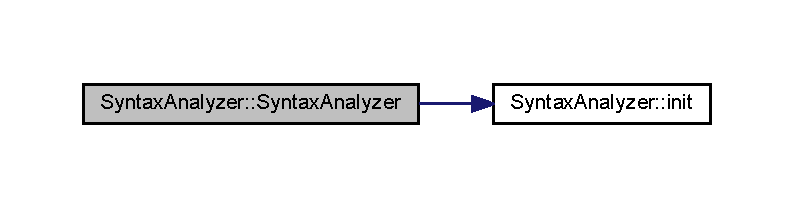
\includegraphics[width=350pt]{class_syntax_analyzer_af4bb6b4b5a638914d5851082dd7a1669_cgraph}
\end{center}
\end{figure}


\index{Syntax\+Analyzer@{Syntax\+Analyzer}!````~Syntax\+Analyzer@{$\sim$\+Syntax\+Analyzer}}
\index{````~Syntax\+Analyzer@{$\sim$\+Syntax\+Analyzer}!Syntax\+Analyzer@{Syntax\+Analyzer}}
\subsubsection[{\texorpdfstring{$\sim$\+Syntax\+Analyzer()}{~SyntaxAnalyzer()}}]{\setlength{\rightskip}{0pt plus 5cm}Syntax\+Analyzer\+::$\sim$\+Syntax\+Analyzer (
\begin{DoxyParamCaption}
{}
\end{DoxyParamCaption}
)\hspace{0.3cm}{\ttfamily [inline]}}\hypertarget{class_syntax_analyzer_a29b52995ad07154244f129673dae5a01}{}\label{class_syntax_analyzer_a29b52995ad07154244f129673dae5a01}


\subsection{Методы}
\index{Syntax\+Analyzer@{Syntax\+Analyzer}!analyze@{analyze}}
\index{analyze@{analyze}!Syntax\+Analyzer@{Syntax\+Analyzer}}
\subsubsection[{\texorpdfstring{analyze()}{analyze()}}]{\setlength{\rightskip}{0pt plus 5cm}vector$<$ {\bf token} $>$ Syntax\+Analyzer\+::analyze (
\begin{DoxyParamCaption}
{}
\end{DoxyParamCaption}
)}\hypertarget{class_syntax_analyzer_a04fbf355b2afe30ef814048ecb029cf2}{}\label{class_syntax_analyzer_a04fbf355b2afe30ef814048ecb029cf2}
Производит синтаксический анализ регулярного выражения

\begin{DoxyReturn}{Возвращает}
Вектор из лексем, который является префиксной записью регулярного выражения 
\end{DoxyReturn}


Граф вызовов\+:
\nopagebreak
\begin{figure}[H]
\begin{center}
\leavevmode
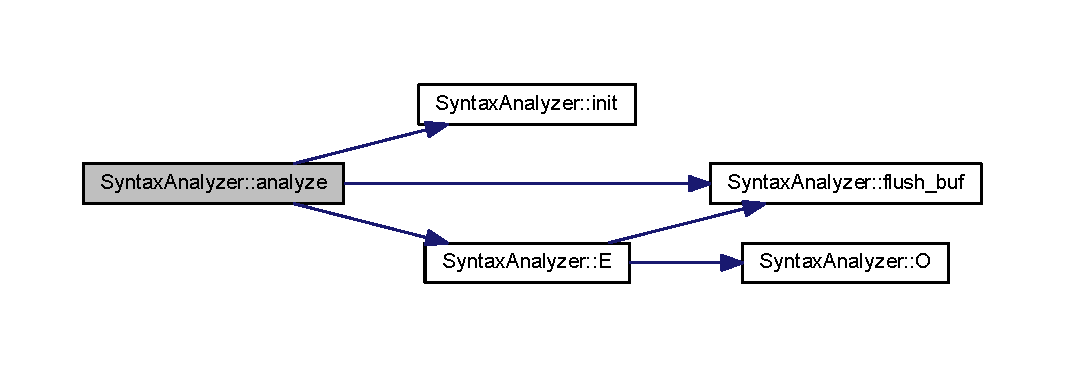
\includegraphics[width=350pt]{class_syntax_analyzer_a04fbf355b2afe30ef814048ecb029cf2_cgraph}
\end{center}
\end{figure}




Граф вызова функции\+:
\nopagebreak
\begin{figure}[H]
\begin{center}
\leavevmode
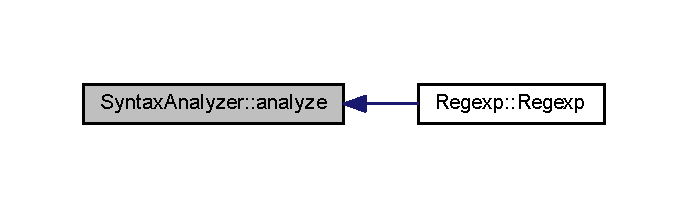
\includegraphics[width=330pt]{class_syntax_analyzer_a04fbf355b2afe30ef814048ecb029cf2_icgraph}
\end{center}
\end{figure}


\index{Syntax\+Analyzer@{Syntax\+Analyzer}!E@{E}}
\index{E@{E}!Syntax\+Analyzer@{Syntax\+Analyzer}}
\subsubsection[{\texorpdfstring{E(bool last=false)}{E(bool last=false)}}]{\setlength{\rightskip}{0pt plus 5cm}void Syntax\+Analyzer\+::E (
\begin{DoxyParamCaption}
\item[{bool}]{last = {\ttfamily false}}
\end{DoxyParamCaption}
)\hspace{0.3cm}{\ttfamily [private]}}\hypertarget{class_syntax_analyzer_a1b42fab3f30284bf29a7eff2f3e8382f}{}\label{class_syntax_analyzer_a1b42fab3f30284bf29a7eff2f3e8382f}
Проверяет выражение и преобразовывает его в префиксную форму 
\begin{DoxyParams}[1]{Аргументы}
\mbox{\tt in}  & {\em last} & Показывает, надо ли останавливаться перед проверкой бинарной операции перечисления \\
\hline
\end{DoxyParams}


Граф вызовов\+:
\nopagebreak
\begin{figure}[H]
\begin{center}
\leavevmode
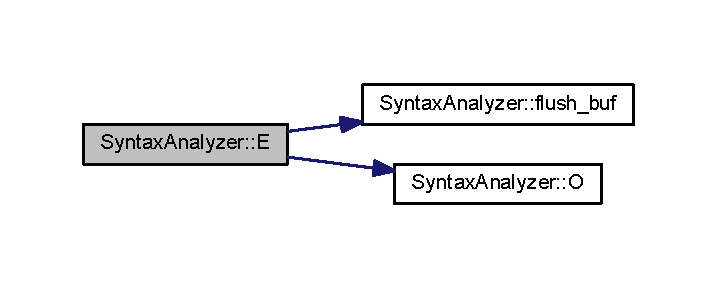
\includegraphics[width=344pt]{class_syntax_analyzer_a1b42fab3f30284bf29a7eff2f3e8382f_cgraph}
\end{center}
\end{figure}




Граф вызова функции\+:
\nopagebreak
\begin{figure}[H]
\begin{center}
\leavevmode
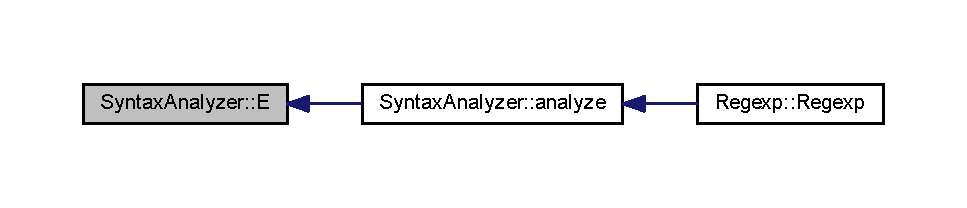
\includegraphics[width=350pt]{class_syntax_analyzer_a1b42fab3f30284bf29a7eff2f3e8382f_icgraph}
\end{center}
\end{figure}


\index{Syntax\+Analyzer@{Syntax\+Analyzer}!flush\+\_\+buf@{flush\+\_\+buf}}
\index{flush\+\_\+buf@{flush\+\_\+buf}!Syntax\+Analyzer@{Syntax\+Analyzer}}
\subsubsection[{\texorpdfstring{flush\+\_\+buf(int pos=-\/1)}{flush_buf(int pos=-1)}}]{\setlength{\rightskip}{0pt plus 5cm}bool Syntax\+Analyzer\+::flush\+\_\+buf (
\begin{DoxyParamCaption}
\item[{int}]{pos = {\ttfamily -\/1}}
\end{DoxyParamCaption}
)\hspace{0.3cm}{\ttfamily [private]}}\hypertarget{class_syntax_analyzer_aea363db29fd359d98711018d377f3301}{}\label{class_syntax_analyzer_aea363db29fd359d98711018d377f3301}
Очищает буфер, занося его содержимое в вектор преобразованных лексем 
\begin{DoxyParams}[1]{Аргументы}
\mbox{\tt in}  & {\em pos} & Позиция, куда необходимо вставить содержимое буфера\\
\hline
\end{DoxyParams}
\begin{DoxyReturn}{Возвращает}
Заполненность буфера на момент вызова 
\end{DoxyReturn}


Граф вызова функции\+:
\nopagebreak
\begin{figure}[H]
\begin{center}
\leavevmode
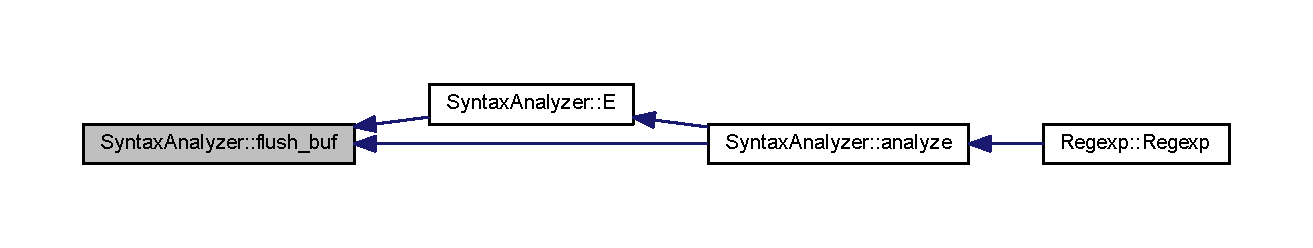
\includegraphics[width=350pt]{class_syntax_analyzer_aea363db29fd359d98711018d377f3301_icgraph}
\end{center}
\end{figure}


\index{Syntax\+Analyzer@{Syntax\+Analyzer}!init@{init}}
\index{init@{init}!Syntax\+Analyzer@{Syntax\+Analyzer}}
\subsubsection[{\texorpdfstring{init()}{init()}}]{\setlength{\rightskip}{0pt plus 5cm}void Syntax\+Analyzer\+::init (
\begin{DoxyParamCaption}
{}
\end{DoxyParamCaption}
)\hspace{0.3cm}{\ttfamily [private]}}\hypertarget{class_syntax_analyzer_a76c8c49d5154b9b48b11d241577420e4}{}\label{class_syntax_analyzer_a76c8c49d5154b9b48b11d241577420e4}


Инициализирует анализатор 



Граф вызова функции\+:
\nopagebreak
\begin{figure}[H]
\begin{center}
\leavevmode
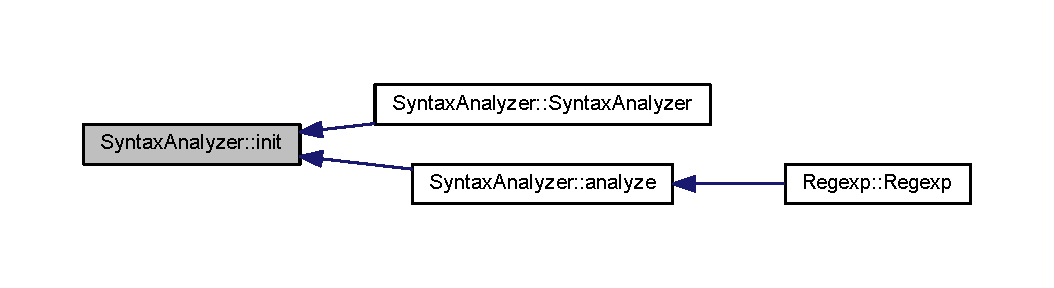
\includegraphics[width=350pt]{class_syntax_analyzer_a76c8c49d5154b9b48b11d241577420e4_icgraph}
\end{center}
\end{figure}


\index{Syntax\+Analyzer@{Syntax\+Analyzer}!O@{O}}
\index{O@{O}!Syntax\+Analyzer@{Syntax\+Analyzer}}
\subsubsection[{\texorpdfstring{O(int pos=-\/1)}{O(int pos=-1)}}]{\setlength{\rightskip}{0pt plus 5cm}bool Syntax\+Analyzer\+::O (
\begin{DoxyParamCaption}
\item[{int}]{pos = {\ttfamily -\/1}}
\end{DoxyParamCaption}
)\hspace{0.3cm}{\ttfamily [private]}}\hypertarget{class_syntax_analyzer_a7a94734bb42224681a23045c45cd9ca3}{}\label{class_syntax_analyzer_a7a94734bb42224681a23045c45cd9ca3}
Проверяет наличие операций и добавляет их в вектор лексем 
\begin{DoxyParams}[1]{Аргументы}
\mbox{\tt in}  & {\em pos} & Позиция, куда необходимо вставить операции\\
\hline
\end{DoxyParams}
\begin{DoxyReturn}{Возвращает}
Наличие операций 
\end{DoxyReturn}


Граф вызова функции\+:
\nopagebreak
\begin{figure}[H]
\begin{center}
\leavevmode
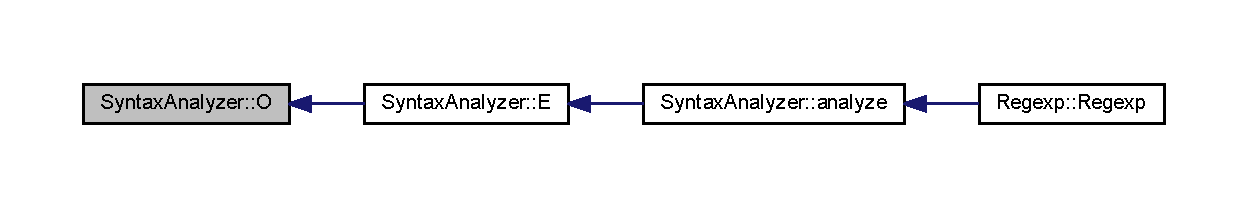
\includegraphics[width=350pt]{class_syntax_analyzer_a7a94734bb42224681a23045c45cd9ca3_icgraph}
\end{center}
\end{figure}




\subsection{Данные класса}
\index{Syntax\+Analyzer@{Syntax\+Analyzer}!brackets\+\_\+count@{brackets\+\_\+count}}
\index{brackets\+\_\+count@{brackets\+\_\+count}!Syntax\+Analyzer@{Syntax\+Analyzer}}
\subsubsection[{\texorpdfstring{brackets\+\_\+count}{brackets_count}}]{\setlength{\rightskip}{0pt plus 5cm}int Syntax\+Analyzer\+::brackets\+\_\+count\hspace{0.3cm}{\ttfamily [private]}}\hypertarget{class_syntax_analyzer_a9ad8571c7819ba91db174772d3fbfbd9}{}\label{class_syntax_analyzer_a9ad8571c7819ba91db174772d3fbfbd9}


Количество незакрытых скобок 

\index{Syntax\+Analyzer@{Syntax\+Analyzer}!buf@{buf}}
\index{buf@{buf}!Syntax\+Analyzer@{Syntax\+Analyzer}}
\subsubsection[{\texorpdfstring{buf}{buf}}]{\setlength{\rightskip}{0pt plus 5cm}string Syntax\+Analyzer\+::buf\hspace{0.3cm}{\ttfamily [private]}}\hypertarget{class_syntax_analyzer_a5b6fe22c4940c5560de49bebe38768e8}{}\label{class_syntax_analyzer_a5b6fe22c4940c5560de49bebe38768e8}


Буфер, используемый для объединения подряд идущих последовательностей литералов 

\index{Syntax\+Analyzer@{Syntax\+Analyzer}!it@{it}}
\index{it@{it}!Syntax\+Analyzer@{Syntax\+Analyzer}}
\subsubsection[{\texorpdfstring{it}{it}}]{\setlength{\rightskip}{0pt plus 5cm}vector$<${\bf token}$>$\+::iterator Syntax\+Analyzer\+::it\hspace{0.3cm}{\ttfamily [private]}}\hypertarget{class_syntax_analyzer_a38e0d3b67ddaa431c1b200f2ad383e61}{}\label{class_syntax_analyzer_a38e0d3b67ddaa431c1b200f2ad383e61}


Итератор, используемый для обхода вектора исходных лексем 

\index{Syntax\+Analyzer@{Syntax\+Analyzer}!pf\+\_\+tokens@{pf\+\_\+tokens}}
\index{pf\+\_\+tokens@{pf\+\_\+tokens}!Syntax\+Analyzer@{Syntax\+Analyzer}}
\subsubsection[{\texorpdfstring{pf\+\_\+tokens}{pf_tokens}}]{\setlength{\rightskip}{0pt plus 5cm}vector$<${\bf token}$>$ Syntax\+Analyzer\+::pf\+\_\+tokens\hspace{0.3cm}{\ttfamily [private]}}\hypertarget{class_syntax_analyzer_aadc7ff59a663670756f4ab5e81f7d99a}{}\label{class_syntax_analyzer_aadc7ff59a663670756f4ab5e81f7d99a}


Вектор с преобразованными лексемами 

\index{Syntax\+Analyzer@{Syntax\+Analyzer}!raw\+\_\+tokens@{raw\+\_\+tokens}}
\index{raw\+\_\+tokens@{raw\+\_\+tokens}!Syntax\+Analyzer@{Syntax\+Analyzer}}
\subsubsection[{\texorpdfstring{raw\+\_\+tokens}{raw_tokens}}]{\setlength{\rightskip}{0pt plus 5cm}vector$<${\bf token}$>$ Syntax\+Analyzer\+::raw\+\_\+tokens\hspace{0.3cm}{\ttfamily [private]}}\hypertarget{class_syntax_analyzer_aea5a27bee70623ed8bf91972938d39af}{}\label{class_syntax_analyzer_aea5a27bee70623ed8bf91972938d39af}


Вектор исходных лексем 



Объявления и описания членов классов находятся в файлах\+:\begin{DoxyCompactItemize}
\item 
\hyperlink{_syntax_analyzer_8h}{Syntax\+Analyzer.\+h}\item 
\hyperlink{_syntax_analyzer_8cpp}{Syntax\+Analyzer.\+cpp}\end{DoxyCompactItemize}

\hypertarget{structtoken}{}\section{Структура token}
\label{structtoken}\index{token@{token}}


Структура лексемы  




{\ttfamily \#include $<$token.\+h$>$}

\subsection*{Открытые атрибуты}
\begin{DoxyCompactItemize}
\item 
\hyperlink{token_8h_afe5ef662303b6b710ea6ee1a944bad0d}{token\+\_\+type} \hyperlink{structtoken_ae4872e33fcec00c59c994c4c9ee3a1f5}{type}
\begin{DoxyCompactList}\small\item\em Тип лексемы \end{DoxyCompactList}\item 
std\+::string \hyperlink{structtoken_a9924c7bd1281e815967e0610dbaeaff1}{lexeme}
\begin{DoxyCompactList}\small\item\em Строковое представление лексемы \end{DoxyCompactList}\end{DoxyCompactItemize}


\subsection{Подробное описание}
Структура лексемы 

\subsection{Данные класса}
\index{token@{token}!lexeme@{lexeme}}
\index{lexeme@{lexeme}!token@{token}}
\subsubsection[{\texorpdfstring{lexeme}{lexeme}}]{\setlength{\rightskip}{0pt plus 5cm}std\+::string token\+::lexeme}\hypertarget{structtoken_a9924c7bd1281e815967e0610dbaeaff1}{}\label{structtoken_a9924c7bd1281e815967e0610dbaeaff1}


Строковое представление лексемы 

\index{token@{token}!type@{type}}
\index{type@{type}!token@{token}}
\subsubsection[{\texorpdfstring{type}{type}}]{\setlength{\rightskip}{0pt plus 5cm}{\bf token\+\_\+type} token\+::type}\hypertarget{structtoken_ae4872e33fcec00c59c994c4c9ee3a1f5}{}\label{structtoken_ae4872e33fcec00c59c994c4c9ee3a1f5}


Тип лексемы 



Объявления и описания членов структуры находятся в файле\+:\begin{DoxyCompactItemize}
\item 
\hyperlink{token_8h}{token.\+h}\end{DoxyCompactItemize}

\chapter{Файлы}
\hypertarget{_lexical_analyzer_8cpp}{}\section{Файл Lexical\+Analyzer.\+cpp}
\label{_lexical_analyzer_8cpp}\index{Lexical\+Analyzer.\+cpp@{Lexical\+Analyzer.\+cpp}}
{\ttfamily \#include \char`\"{}Lexical\+Analyzer.\+h\char`\"{}}\\*
Граф включаемых заголовочных файлов для Lexical\+Analyzer.\+cpp\+:
\nopagebreak
\begin{figure}[H]
\begin{center}
\leavevmode
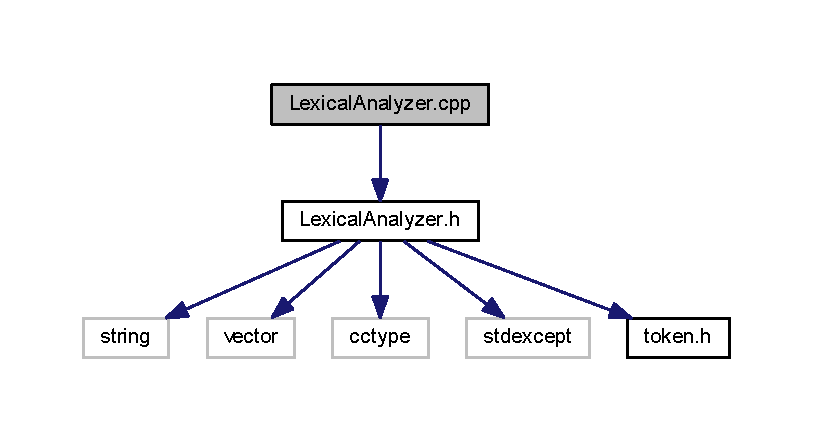
\includegraphics[width=350pt]{_lexical_analyzer_8cpp__incl}
\end{center}
\end{figure}

\hypertarget{_lexical_analyzer_8h}{}\section{Файл Lexical\+Analyzer.\+h}
\label{_lexical_analyzer_8h}\index{Lexical\+Analyzer.\+h@{Lexical\+Analyzer.\+h}}


Заголовочный файл лексического анализатора  


{\ttfamily \#include $<$string$>$}\\*
{\ttfamily \#include $<$vector$>$}\\*
{\ttfamily \#include $<$cctype$>$}\\*
{\ttfamily \#include $<$stdexcept$>$}\\*
{\ttfamily \#include \char`\"{}token.\+h\char`\"{}}\\*
Граф включаемых заголовочных файлов для Lexical\+Analyzer.\+h\+:
\nopagebreak
\begin{figure}[H]
\begin{center}
\leavevmode
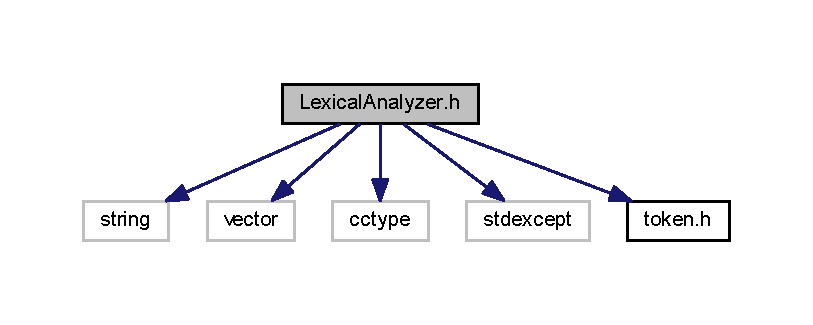
\includegraphics[width=350pt]{_lexical_analyzer_8h__incl}
\end{center}
\end{figure}
Граф файлов, в которые включается этот файл\+:
\nopagebreak
\begin{figure}[H]
\begin{center}
\leavevmode
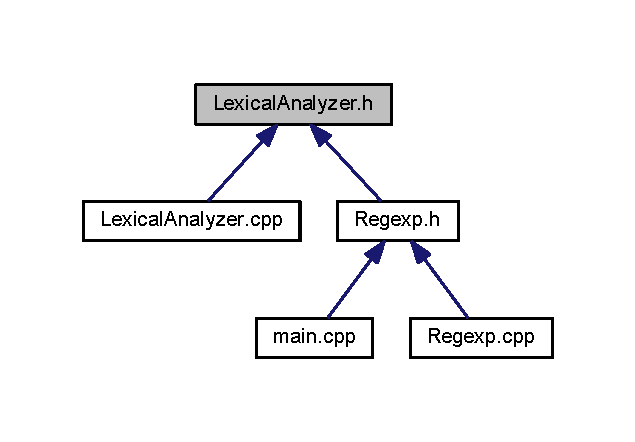
\includegraphics[width=305pt]{_lexical_analyzer_8h__dep__incl}
\end{center}
\end{figure}
\subsection*{Классы}
\begin{DoxyCompactItemize}
\item 
class \hyperlink{class_lexical_analyzer}{Lexical\+Analyzer}
\begin{DoxyCompactList}\small\item\em Лексический анализатор \end{DoxyCompactList}\end{DoxyCompactItemize}


\subsection{Подробное описание}
Заголовочный файл лексического анализатора 

\begin{DoxyAuthor}{Автор}
Invalid\+Pointer
\end{DoxyAuthor}
Данный файл содержит в себе определение класса лексического анализатора 
\hypertarget{main_8cpp}{}\section{Файл main.\+cpp}
\label{main_8cpp}\index{main.\+cpp@{main.\+cpp}}
{\ttfamily \#include $<$iostream$>$}\\*
{\ttfamily \#include $<$cstring$>$}\\*
{\ttfamily \#include \char`\"{}Regexp.\+h\char`\"{}}\\*
Граф включаемых заголовочных файлов для main.\+cpp\+:
\nopagebreak
\begin{figure}[H]
\begin{center}
\leavevmode
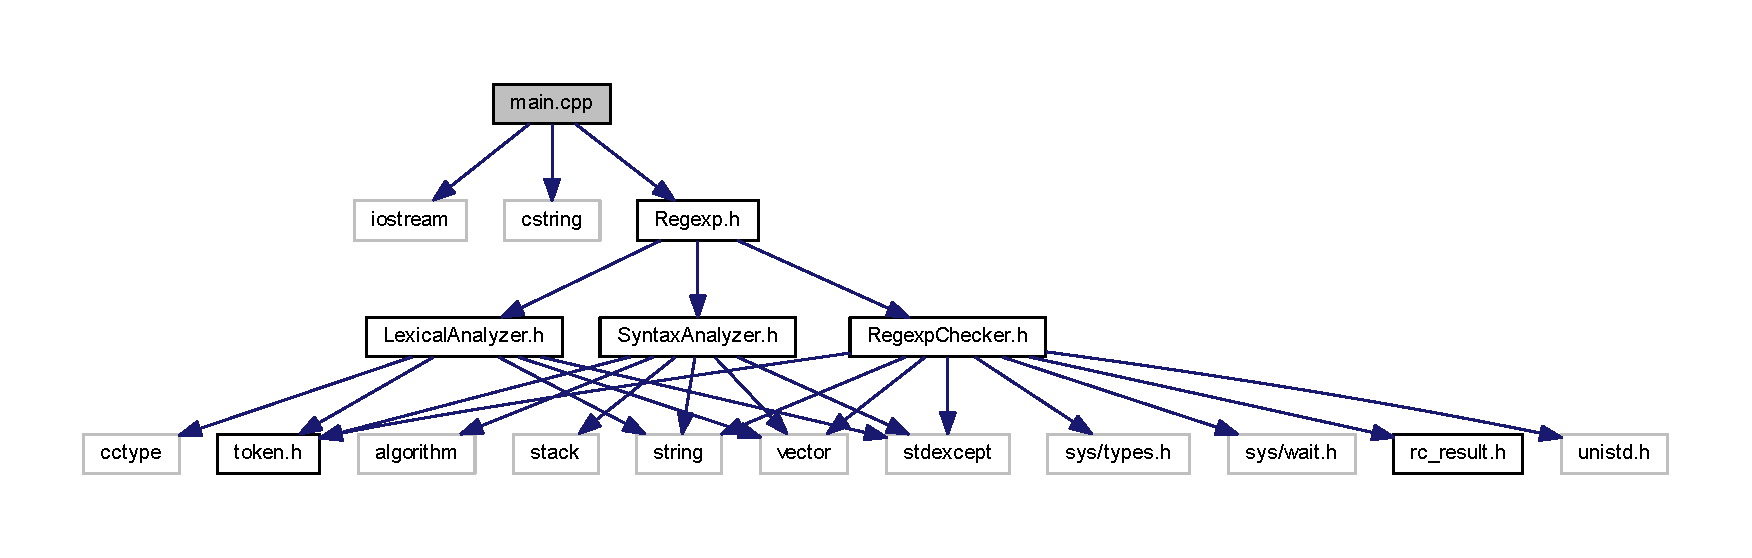
\includegraphics[width=350pt]{main_8cpp__incl}
\end{center}
\end{figure}
\subsection*{Функции}
\begin{DoxyCompactItemize}
\item 
int \hyperlink{main_8cpp_a3c04138a5bfe5d72780bb7e82a18e627}{main} (int argc, char $\ast$$\ast$argv)
\end{DoxyCompactItemize}


\subsection{Функции}
\index{main.\+cpp@{main.\+cpp}!main@{main}}
\index{main@{main}!main.\+cpp@{main.\+cpp}}
\subsubsection[{\texorpdfstring{main(int argc, char $\ast$$\ast$argv)}{main(int argc, char **argv)}}]{\setlength{\rightskip}{0pt plus 5cm}int main (
\begin{DoxyParamCaption}
\item[{int}]{argc, }
\item[{char $\ast$$\ast$}]{argv}
\end{DoxyParamCaption}
)}\hypertarget{main_8cpp_a3c04138a5bfe5d72780bb7e82a18e627}{}\label{main_8cpp_a3c04138a5bfe5d72780bb7e82a18e627}


Граф вызовов\+:
\nopagebreak
\begin{figure}[H]
\begin{center}
\leavevmode
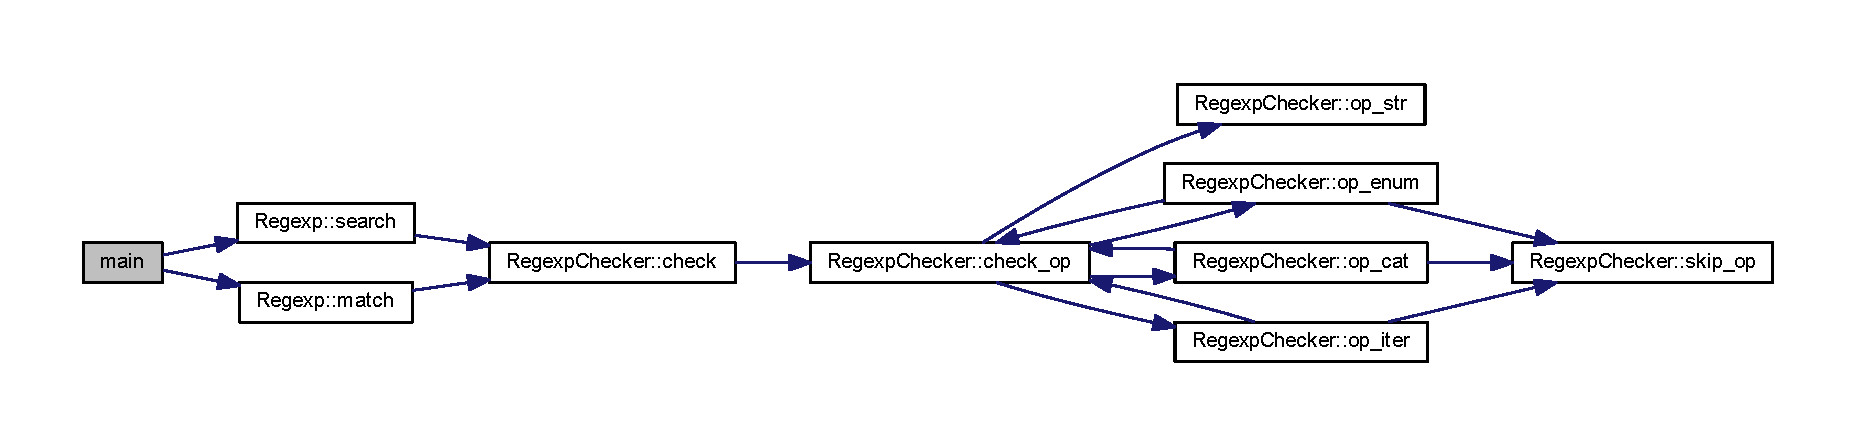
\includegraphics[width=350pt]{main_8cpp_a3c04138a5bfe5d72780bb7e82a18e627_cgraph}
\end{center}
\end{figure}



\hypertarget{rc__result_8h}{}\section{Файл rc\+\_\+result.\+h}
\label{rc__result_8h}\index{rc\+\_\+result.\+h@{rc\+\_\+result.\+h}}


Файл с определением результата работы класса проверки строк  


Граф файлов, в которые включается этот файл\+:
\nopagebreak
\begin{figure}[H]
\begin{center}
\leavevmode
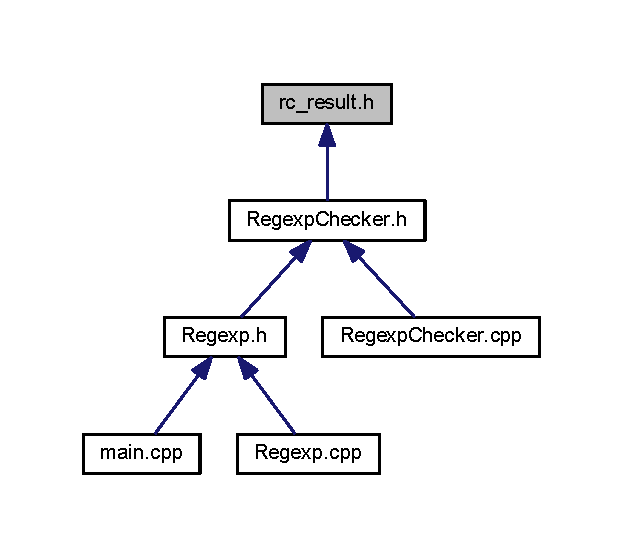
\includegraphics[width=299pt]{rc__result_8h__dep__incl}
\end{center}
\end{figure}
\subsection*{Классы}
\begin{DoxyCompactItemize}
\item 
struct \hyperlink{structrc__result}{rc\+\_\+result}
\begin{DoxyCompactList}\small\item\em Структура, описывающая формат результата \end{DoxyCompactList}\end{DoxyCompactItemize}


\subsection{Подробное описание}
Файл с определением результата работы класса проверки строк 

\begin{DoxyAuthor}{Автор}
Invalid\+Pointer
\end{DoxyAuthor}
Данный файл содержит в себе определение структуры, используемой классом проверки регулярных выражений 
\hypertarget{_regexp_8cpp}{}\section{Файл Regexp.\+cpp}
\label{_regexp_8cpp}\index{Regexp.\+cpp@{Regexp.\+cpp}}
{\ttfamily \#include $<$iostream$>$}\\*
{\ttfamily \#include \char`\"{}Regexp.\+h\char`\"{}}\\*
Граф включаемых заголовочных файлов для Regexp.\+cpp\+:
\nopagebreak
\begin{figure}[H]
\begin{center}
\leavevmode
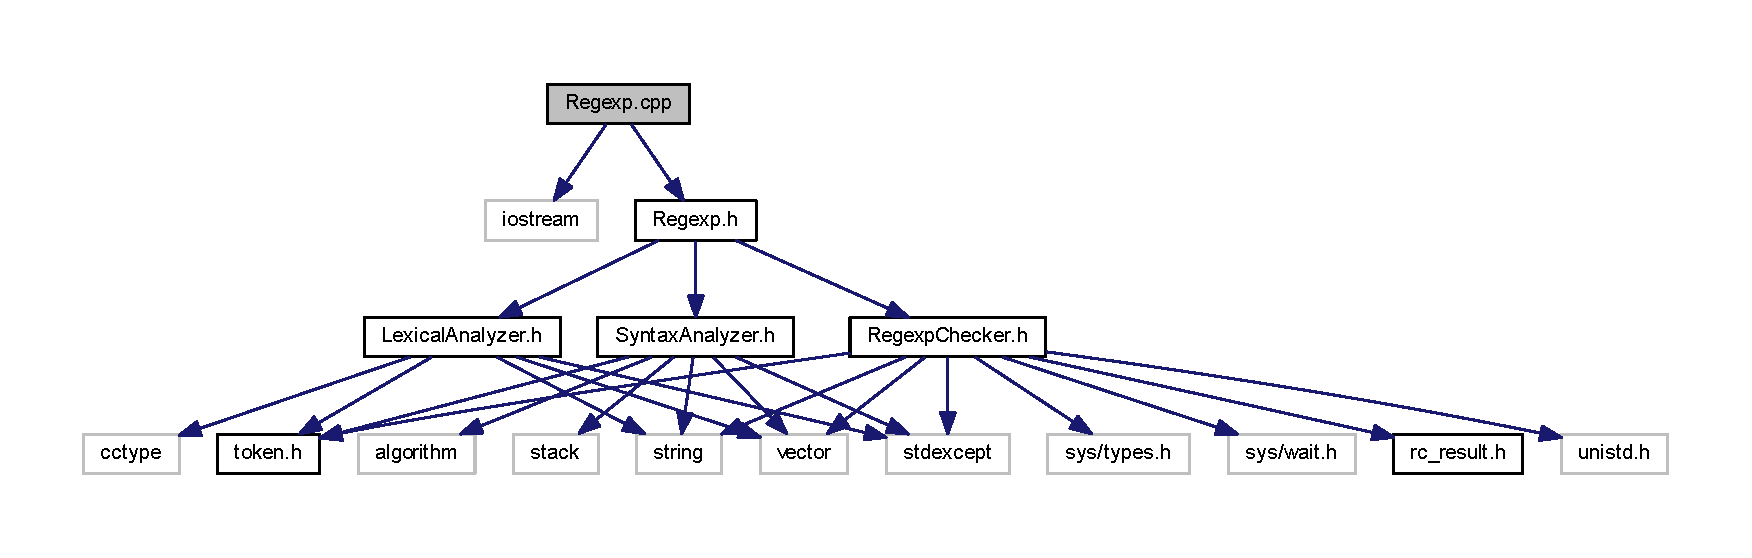
\includegraphics[width=350pt]{_regexp_8cpp__incl}
\end{center}
\end{figure}

\hypertarget{_regexp_8h}{}\section{Файл Regexp.\+h}
\label{_regexp_8h}\index{Regexp.\+h@{Regexp.\+h}}


Заголовочный файл класса регулярного выражения  


{\ttfamily \#include \char`\"{}Lexical\+Analyzer.\+h\char`\"{}}\\*
{\ttfamily \#include \char`\"{}Syntax\+Analyzer.\+h\char`\"{}}\\*
{\ttfamily \#include \char`\"{}Regexp\+Checker.\+h\char`\"{}}\\*
Граф включаемых заголовочных файлов для Regexp.\+h\+:
\nopagebreak
\begin{figure}[H]
\begin{center}
\leavevmode
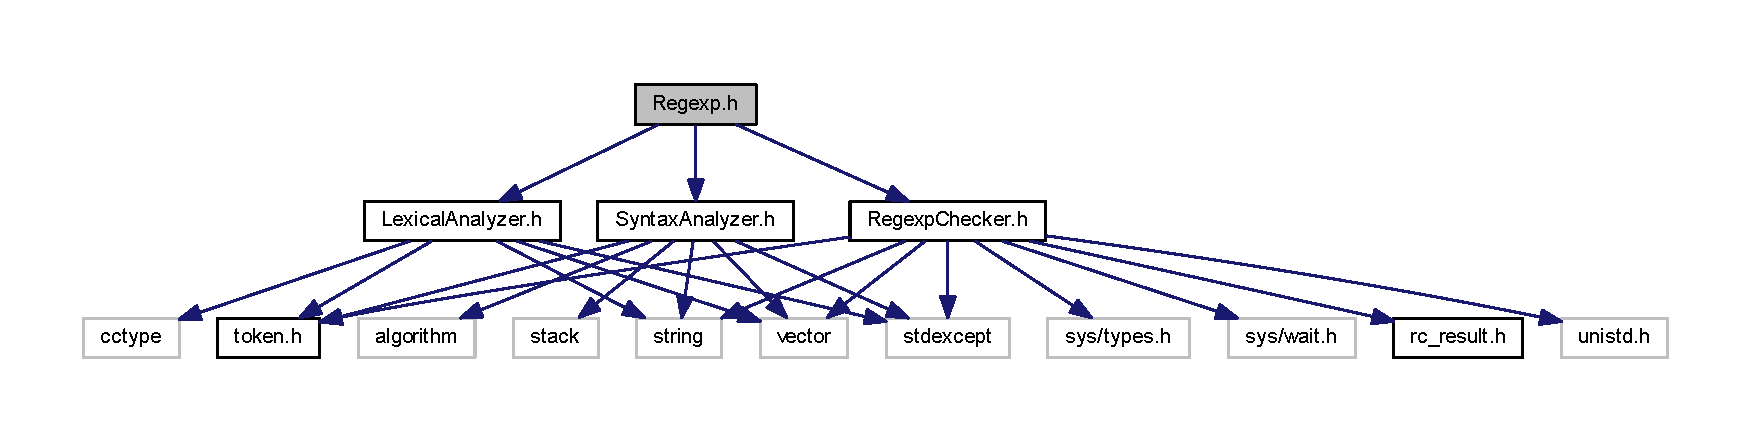
\includegraphics[width=350pt]{_regexp_8h__incl}
\end{center}
\end{figure}
Граф файлов, в которые включается этот файл\+:
\nopagebreak
\begin{figure}[H]
\begin{center}
\leavevmode
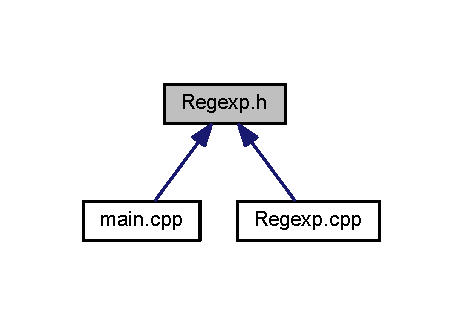
\includegraphics[width=222pt]{_regexp_8h__dep__incl}
\end{center}
\end{figure}
\subsection*{Классы}
\begin{DoxyCompactItemize}
\item 
class \hyperlink{class_regexp}{Regexp}
\begin{DoxyCompactList}\small\item\em Класс регулярного выражения \end{DoxyCompactList}\end{DoxyCompactItemize}


\subsection{Подробное описание}
Заголовочный файл класса регулярного выражения 

\begin{DoxyAuthor}{Автор}
Invalid\+Pointer
\end{DoxyAuthor}
Данный файл содержит в себе определение класса, в котором реализованы обёртки над классом, занимающимся проверкой строк, в виде функций \hyperlink{class_regexp_a7869806d5707d47742db7ad5129b6585}{Regexp\+::match()} и \hyperlink{class_regexp_af7c296f94f7577ce0fa662c78268659e}{Regexp\+::search()} 
\hypertarget{_regexp_checker_8cpp}{}\section{Файл Regexp\+Checker.\+cpp}
\label{_regexp_checker_8cpp}\index{Regexp\+Checker.\+cpp@{Regexp\+Checker.\+cpp}}
{\ttfamily \#include \char`\"{}Regexp\+Checker.\+h\char`\"{}}\\*
Граф включаемых заголовочных файлов для Regexp\+Checker.\+cpp\+:
\nopagebreak
\begin{figure}[H]
\begin{center}
\leavevmode
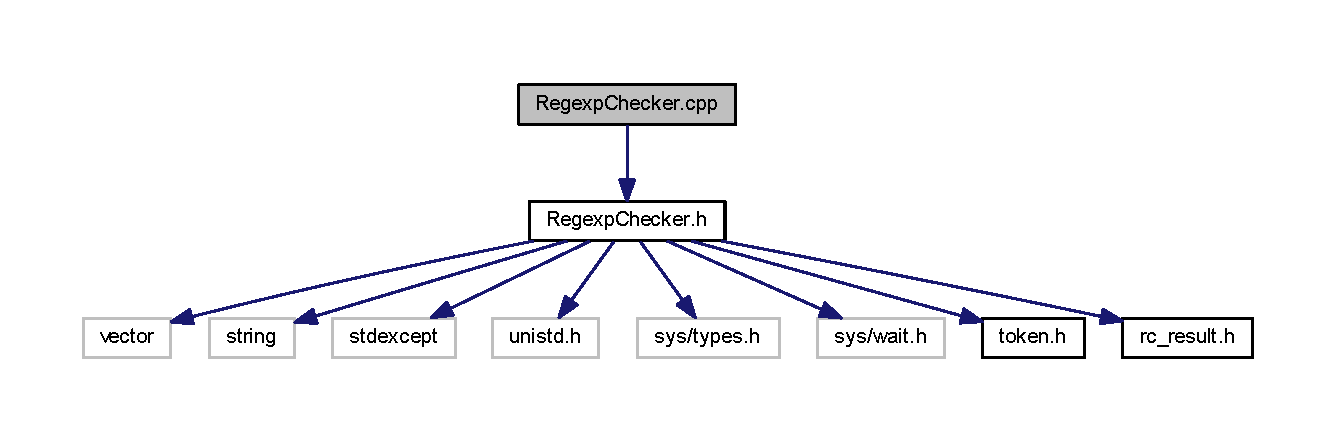
\includegraphics[width=350pt]{_regexp_checker_8cpp__incl}
\end{center}
\end{figure}

\hypertarget{_regexp_checker_8h}{}\section{Файл Regexp\+Checker.\+h}
\label{_regexp_checker_8h}\index{Regexp\+Checker.\+h@{Regexp\+Checker.\+h}}


Заголовочный файл класса, проверяющего строки  


{\ttfamily \#include $<$vector$>$}\\*
{\ttfamily \#include $<$string$>$}\\*
{\ttfamily \#include $<$stdexcept$>$}\\*
{\ttfamily \#include $<$unistd.\+h$>$}\\*
{\ttfamily \#include $<$sys/types.\+h$>$}\\*
{\ttfamily \#include $<$sys/wait.\+h$>$}\\*
{\ttfamily \#include \char`\"{}token.\+h\char`\"{}}\\*
{\ttfamily \#include \char`\"{}rc\+\_\+result.\+h\char`\"{}}\\*
Граф включаемых заголовочных файлов для Regexp\+Checker.\+h\+:
\nopagebreak
\begin{figure}[H]
\begin{center}
\leavevmode
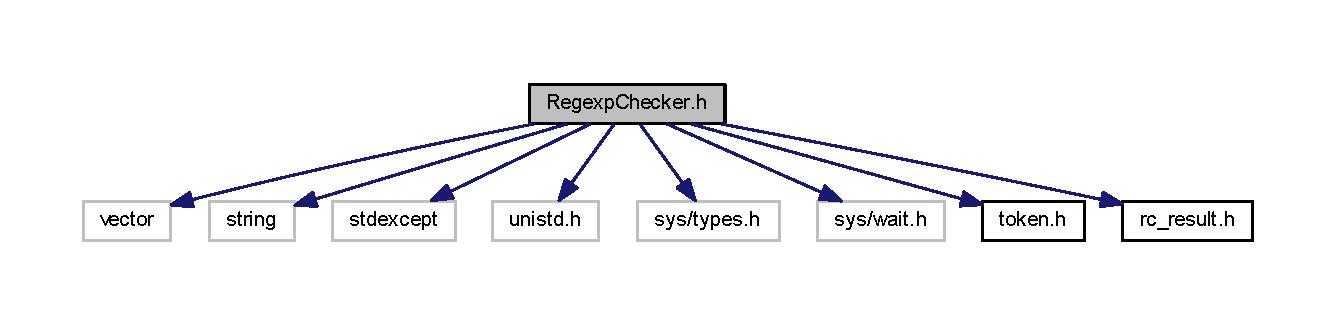
\includegraphics[width=350pt]{_regexp_checker_8h__incl}
\end{center}
\end{figure}
Граф файлов, в которые включается этот файл\+:
\nopagebreak
\begin{figure}[H]
\begin{center}
\leavevmode
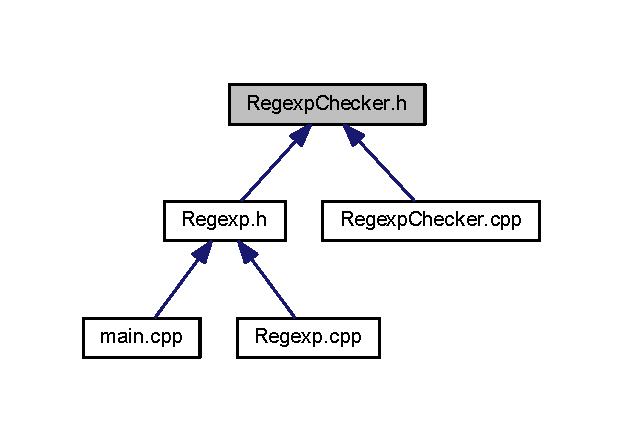
\includegraphics[width=299pt]{_regexp_checker_8h__dep__incl}
\end{center}
\end{figure}
\subsection*{Классы}
\begin{DoxyCompactItemize}
\item 
class \hyperlink{class_regexp_checker}{Regexp\+Checker}
\begin{DoxyCompactList}\small\item\em Класс, проверяющий строку на соответствие регулярному выражению \end{DoxyCompactList}\end{DoxyCompactItemize}


\subsection{Подробное описание}
Заголовочный файл класса, проверяющего строки 

\begin{DoxyAuthor}{Автор}
Invalid\+Pointer
\end{DoxyAuthor}
Данный файл содержит в себе определение класса, который реализует механизм проверки соответствия строки с регулярным выражнием 
\hypertarget{_syntax_analyzer_8cpp}{}\section{Файл Syntax\+Analyzer.\+cpp}
\label{_syntax_analyzer_8cpp}\index{Syntax\+Analyzer.\+cpp@{Syntax\+Analyzer.\+cpp}}
{\ttfamily \#include \char`\"{}Syntax\+Analyzer.\+h\char`\"{}}\\*
Граф включаемых заголовочных файлов для Syntax\+Analyzer.\+cpp\+:
\nopagebreak
\begin{figure}[H]
\begin{center}
\leavevmode
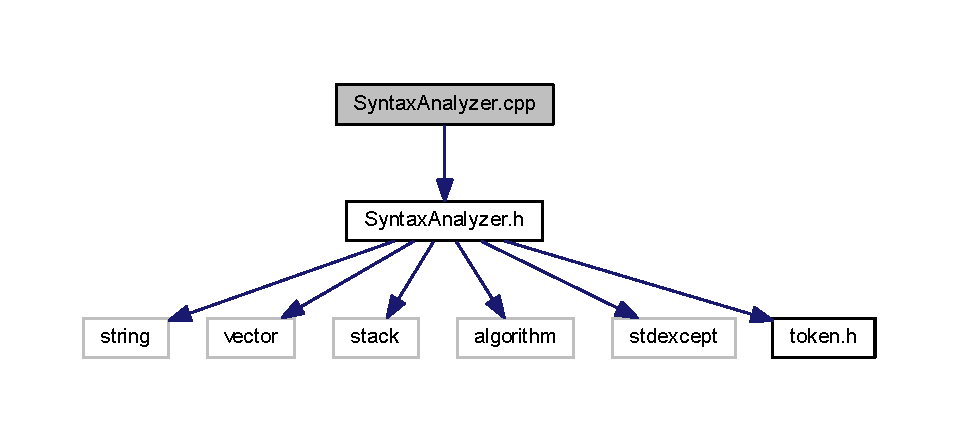
\includegraphics[width=350pt]{_syntax_analyzer_8cpp__incl}
\end{center}
\end{figure}

\hypertarget{_syntax_analyzer_8h}{}\section{Файл Syntax\+Analyzer.\+h}
\label{_syntax_analyzer_8h}\index{Syntax\+Analyzer.\+h@{Syntax\+Analyzer.\+h}}


Заголовочный файл синтаксического анализатора  


{\ttfamily \#include $<$string$>$}\\*
{\ttfamily \#include $<$vector$>$}\\*
{\ttfamily \#include $<$stack$>$}\\*
{\ttfamily \#include $<$algorithm$>$}\\*
{\ttfamily \#include $<$stdexcept$>$}\\*
{\ttfamily \#include \char`\"{}token.\+h\char`\"{}}\\*
Граф включаемых заголовочных файлов для Syntax\+Analyzer.\+h\+:
\nopagebreak
\begin{figure}[H]
\begin{center}
\leavevmode
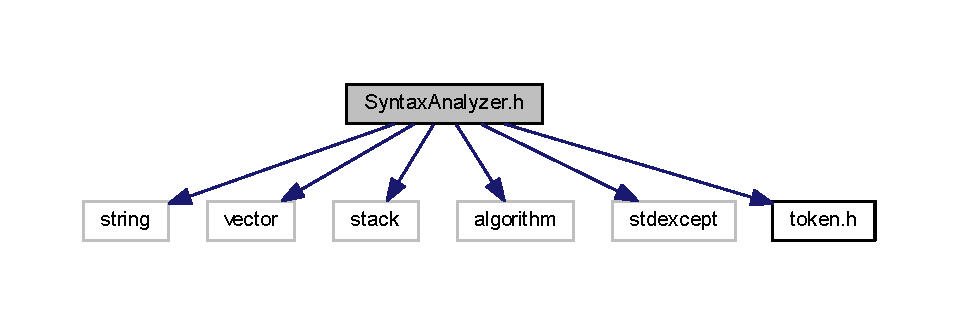
\includegraphics[width=350pt]{_syntax_analyzer_8h__incl}
\end{center}
\end{figure}
Граф файлов, в которые включается этот файл\+:
\nopagebreak
\begin{figure}[H]
\begin{center}
\leavevmode
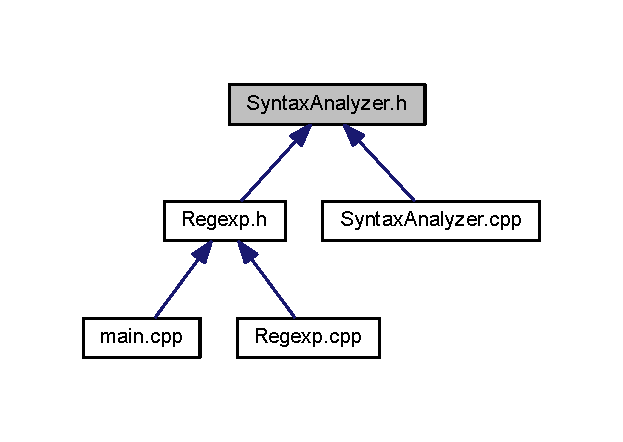
\includegraphics[width=299pt]{_syntax_analyzer_8h__dep__incl}
\end{center}
\end{figure}
\subsection*{Классы}
\begin{DoxyCompactItemize}
\item 
class \hyperlink{class_syntax_analyzer}{Syntax\+Analyzer}
\begin{DoxyCompactList}\small\item\em Синтаксический анализатор \end{DoxyCompactList}\end{DoxyCompactItemize}


\subsection{Подробное описание}
Заголовочный файл синтаксического анализатора 

\begin{DoxyAuthor}{Автор}
Invalid\+Pointer
\end{DoxyAuthor}
Данный файл содержит в себе определение класса синтаксического анализатора

Грамматика, которую использует анализатор\+: E -\/$>$ (E)O $\vert$ EE $\vert$ \{literal\}O $\vert$ E$|$E O -\/$>$ $\ast$O $\vert$ \{,n\}O $\vert$ \{m,\}O $\vert$ \+\_\+ 
\hypertarget{token_8h}{}\section{Файл token.\+h}
\label{token_8h}\index{token.\+h@{token.\+h}}


Файл с определением структуры лексемы  


Граф файлов, в которые включается этот файл\+:
\nopagebreak
\begin{figure}[H]
\begin{center}
\leavevmode
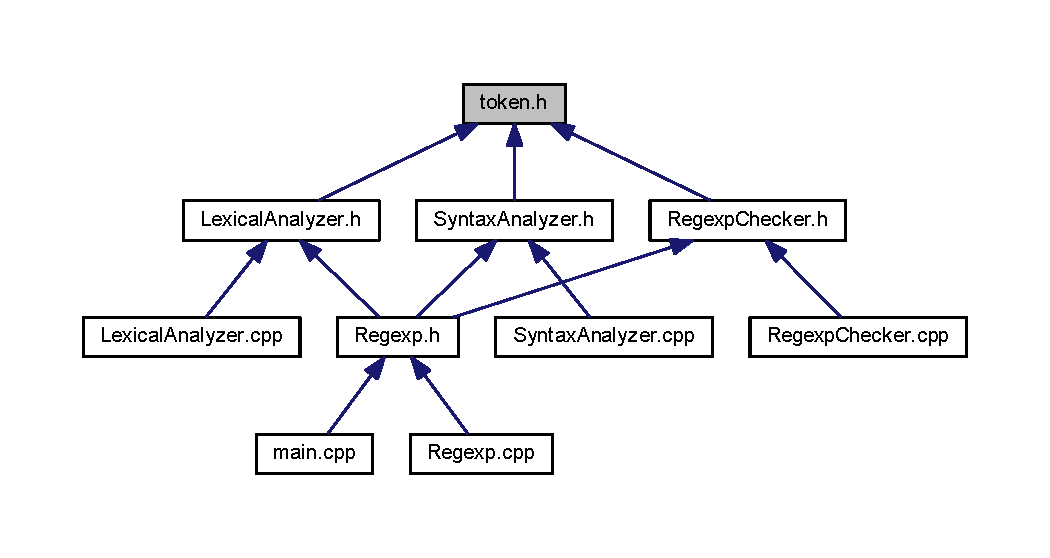
\includegraphics[width=350pt]{token_8h__dep__incl}
\end{center}
\end{figure}
\subsection*{Классы}
\begin{DoxyCompactItemize}
\item 
struct \hyperlink{structtoken}{token}
\begin{DoxyCompactList}\small\item\em Структура лексемы \end{DoxyCompactList}\end{DoxyCompactItemize}
\subsection*{Перечисления}
\begin{DoxyCompactItemize}
\item 
enum \hyperlink{token_8h_afe5ef662303b6b710ea6ee1a944bad0d}{token\+\_\+type} \{ \\*
\hyperlink{token_8h_afe5ef662303b6b710ea6ee1a944bad0da3fef8bbb5f93d143a64514ef24fcf6d4}{O\+\_\+\+B\+R\+\_\+T}, 
\hyperlink{token_8h_afe5ef662303b6b710ea6ee1a944bad0da2f8419e4924ed901fea345a477f57099}{C\+\_\+\+B\+R\+\_\+T}, 
\hyperlink{token_8h_afe5ef662303b6b710ea6ee1a944bad0da19986f9d7a7a4490063a73769c71dea2}{E\+N\+U\+M\+\_\+T}, 
\hyperlink{token_8h_afe5ef662303b6b710ea6ee1a944bad0da361569a0a02c73a6b3c61d8120c55822}{S\+T\+R\+\_\+T}, 
\\*
\hyperlink{token_8h_afe5ef662303b6b710ea6ee1a944bad0daa65d2890d1cf384b5570002835722c12}{C\+A\+T\+\_\+T}, 
\hyperlink{token_8h_afe5ef662303b6b710ea6ee1a944bad0dad117e84ed28d908e6853db06779e913e}{I\+T\+E\+R\+\_\+\+Z\+O\+\_\+T}, 
\hyperlink{token_8h_afe5ef662303b6b710ea6ee1a944bad0dac7613bf6d065d7465e4325704f9adcb7}{I\+T\+E\+R\+\_\+\+O\+M\+\_\+T}, 
\hyperlink{token_8h_afe5ef662303b6b710ea6ee1a944bad0da8de1f797d0d39e201c2aa538affc9f88}{I\+T\+E\+R\+\_\+\+Z\+M\+\_\+T}, 
\\*
\hyperlink{token_8h_afe5ef662303b6b710ea6ee1a944bad0dabcd8de3a261c1dde58c0de1ce00d3cab}{I\+T\+E\+R\+\_\+\+N\+\_\+T}
 \}\begin{DoxyCompactList}\small\item\em Тип лексемы \end{DoxyCompactList}
\end{DoxyCompactItemize}
\subsection*{Переменные}
\begin{DoxyCompactItemize}
\item 
const int \hyperlink{token_8h_a720268725b243dc6376e8247009df4af}{prior} \mbox{[}$\,$\mbox{]} = \{0, 0, 1, 2, 2, 3, 3, 3, 3\}
\begin{DoxyCompactList}\small\item\em Приоритеты операций, в порядке описанном выше \end{DoxyCompactList}\end{DoxyCompactItemize}


\subsection{Подробное описание}
Файл с определением структуры лексемы 

\begin{DoxyAuthor}{Автор}
Invalid\+Pointer
\end{DoxyAuthor}
Данный файл содержит в себе определение структуры лексемы, их типы и приоритеты 

\subsection{Перечисления}
\index{token.\+h@{token.\+h}!token\+\_\+type@{token\+\_\+type}}
\index{token\+\_\+type@{token\+\_\+type}!token.\+h@{token.\+h}}
\subsubsection[{\texorpdfstring{token\+\_\+type}{token_type}}]{\setlength{\rightskip}{0pt plus 5cm}enum {\bf token\+\_\+type}}\hypertarget{token_8h_afe5ef662303b6b710ea6ee1a944bad0d}{}\label{token_8h_afe5ef662303b6b710ea6ee1a944bad0d}


Тип лексемы 

\begin{Desc}
\item[Элементы перечислений]\par
\begin{description}
\index{O\+\_\+\+B\+R\+\_\+T@{O\+\_\+\+B\+R\+\_\+T}!token.\+h@{token.\+h}}\index{token.\+h@{token.\+h}!O\+\_\+\+B\+R\+\_\+T@{O\+\_\+\+B\+R\+\_\+T}}\item[{\em 
O\+\_\+\+B\+R\+\_\+T\hypertarget{token_8h_afe5ef662303b6b710ea6ee1a944bad0da3fef8bbb5f93d143a64514ef24fcf6d4}{}\label{token_8h_afe5ef662303b6b710ea6ee1a944bad0da3fef8bbb5f93d143a64514ef24fcf6d4}
}]Открывающая скобка \index{C\+\_\+\+B\+R\+\_\+T@{C\+\_\+\+B\+R\+\_\+T}!token.\+h@{token.\+h}}\index{token.\+h@{token.\+h}!C\+\_\+\+B\+R\+\_\+T@{C\+\_\+\+B\+R\+\_\+T}}\item[{\em 
C\+\_\+\+B\+R\+\_\+T\hypertarget{token_8h_afe5ef662303b6b710ea6ee1a944bad0da2f8419e4924ed901fea345a477f57099}{}\label{token_8h_afe5ef662303b6b710ea6ee1a944bad0da2f8419e4924ed901fea345a477f57099}
}]Закрывающая скобка \index{E\+N\+U\+M\+\_\+T@{E\+N\+U\+M\+\_\+T}!token.\+h@{token.\+h}}\index{token.\+h@{token.\+h}!E\+N\+U\+M\+\_\+T@{E\+N\+U\+M\+\_\+T}}\item[{\em 
E\+N\+U\+M\+\_\+T\hypertarget{token_8h_afe5ef662303b6b710ea6ee1a944bad0da19986f9d7a7a4490063a73769c71dea2}{}\label{token_8h_afe5ef662303b6b710ea6ee1a944bad0da19986f9d7a7a4490063a73769c71dea2}
}]Операция перечисления \index{S\+T\+R\+\_\+T@{S\+T\+R\+\_\+T}!token.\+h@{token.\+h}}\index{token.\+h@{token.\+h}!S\+T\+R\+\_\+T@{S\+T\+R\+\_\+T}}\item[{\em 
S\+T\+R\+\_\+T\hypertarget{token_8h_afe5ef662303b6b710ea6ee1a944bad0da361569a0a02c73a6b3c61d8120c55822}{}\label{token_8h_afe5ef662303b6b710ea6ee1a944bad0da361569a0a02c73a6b3c61d8120c55822}
}]Литерал или последовательность литералов \index{C\+A\+T\+\_\+T@{C\+A\+T\+\_\+T}!token.\+h@{token.\+h}}\index{token.\+h@{token.\+h}!C\+A\+T\+\_\+T@{C\+A\+T\+\_\+T}}\item[{\em 
C\+A\+T\+\_\+T\hypertarget{token_8h_afe5ef662303b6b710ea6ee1a944bad0daa65d2890d1cf384b5570002835722c12}{}\label{token_8h_afe5ef662303b6b710ea6ee1a944bad0daa65d2890d1cf384b5570002835722c12}
}]Операция конкатенации \index{I\+T\+E\+R\+\_\+\+Z\+O\+\_\+T@{I\+T\+E\+R\+\_\+\+Z\+O\+\_\+T}!token.\+h@{token.\+h}}\index{token.\+h@{token.\+h}!I\+T\+E\+R\+\_\+\+Z\+O\+\_\+T@{I\+T\+E\+R\+\_\+\+Z\+O\+\_\+T}}\item[{\em 
I\+T\+E\+R\+\_\+\+Z\+O\+\_\+T\hypertarget{token_8h_afe5ef662303b6b710ea6ee1a944bad0dad117e84ed28d908e6853db06779e913e}{}\label{token_8h_afe5ef662303b6b710ea6ee1a944bad0dad117e84ed28d908e6853db06779e913e}
}]Операция итерирования 0 или 1 раз \index{I\+T\+E\+R\+\_\+\+O\+M\+\_\+T@{I\+T\+E\+R\+\_\+\+O\+M\+\_\+T}!token.\+h@{token.\+h}}\index{token.\+h@{token.\+h}!I\+T\+E\+R\+\_\+\+O\+M\+\_\+T@{I\+T\+E\+R\+\_\+\+O\+M\+\_\+T}}\item[{\em 
I\+T\+E\+R\+\_\+\+O\+M\+\_\+T\hypertarget{token_8h_afe5ef662303b6b710ea6ee1a944bad0dac7613bf6d065d7465e4325704f9adcb7}{}\label{token_8h_afe5ef662303b6b710ea6ee1a944bad0dac7613bf6d065d7465e4325704f9adcb7}
}]Операция итерирования 1 или более раз \index{I\+T\+E\+R\+\_\+\+Z\+M\+\_\+T@{I\+T\+E\+R\+\_\+\+Z\+M\+\_\+T}!token.\+h@{token.\+h}}\index{token.\+h@{token.\+h}!I\+T\+E\+R\+\_\+\+Z\+M\+\_\+T@{I\+T\+E\+R\+\_\+\+Z\+M\+\_\+T}}\item[{\em 
I\+T\+E\+R\+\_\+\+Z\+M\+\_\+T\hypertarget{token_8h_afe5ef662303b6b710ea6ee1a944bad0da8de1f797d0d39e201c2aa538affc9f88}{}\label{token_8h_afe5ef662303b6b710ea6ee1a944bad0da8de1f797d0d39e201c2aa538affc9f88}
}]Операция итерирования 0 или более раз \index{I\+T\+E\+R\+\_\+\+N\+\_\+T@{I\+T\+E\+R\+\_\+\+N\+\_\+T}!token.\+h@{token.\+h}}\index{token.\+h@{token.\+h}!I\+T\+E\+R\+\_\+\+N\+\_\+T@{I\+T\+E\+R\+\_\+\+N\+\_\+T}}\item[{\em 
I\+T\+E\+R\+\_\+\+N\+\_\+T\hypertarget{token_8h_afe5ef662303b6b710ea6ee1a944bad0dabcd8de3a261c1dde58c0de1ce00d3cab}{}\label{token_8h_afe5ef662303b6b710ea6ee1a944bad0dabcd8de3a261c1dde58c0de1ce00d3cab}
}]Операция итерирования \end{description}
\end{Desc}


\subsection{Переменные}
\index{token.\+h@{token.\+h}!prior@{prior}}
\index{prior@{prior}!token.\+h@{token.\+h}}
\subsubsection[{\texorpdfstring{prior}{prior}}]{\setlength{\rightskip}{0pt plus 5cm}const int prior\mbox{[}$\,$\mbox{]} = \{0, 0, 1, 2, 2, 3, 3, 3, 3\}}\hypertarget{token_8h_a720268725b243dc6376e8247009df4af}{}\label{token_8h_a720268725b243dc6376e8247009df4af}


Приоритеты операций, в порядке описанном выше 


%--- End generated contents ---

% Index
\backmatter
\newpage
\phantomsection
\clearemptydoublepage
\addcontentsline{toc}{chapter}{Алфавитный указатель}
\printindex

\end{document}
